\documentclass[11pt]{article}

\usepackage[a4paper,margin=1in]{geometry}
\usepackage[T1]{fontenc}
\usepackage[utf8]{inputenc}
\usepackage{lmodern}
\usepackage{amsmath,amssymb,bm}
\usepackage{booktabs}
\usepackage{array}
\usepackage{tabularx}
\usepackage{graphicx}
\usepackage{xcolor}
\usepackage{microtype}
\usepackage{cite}
\usepackage[hidelinks]{hyperref}
\usepackage{authblk}
\usepackage{float}
\usepackage[section,above,below]{placeins}
\usepackage[font=small,labelfont=bf]{caption}
\captionsetup[figure]{name=Figure,labelsep=colon}
\usepackage{fancyhdr}
\pagestyle{fancy}
\fancyhf{}
\cfoot{\thepage}
\renewcommand{\headrulewidth}{0pt}
\renewcommand{\footrulewidth}{0pt}
\fancypagestyle{plain}{
  \fancyhf{}
  \cfoot{\thepage}
  \renewcommand{\headrulewidth}{0pt}
  \renewcommand{\footrulewidth}{0pt}
}

\graphicspath{{figures/}}
\hypersetup{
  pdftitle={A Geometric Criterion for Sway and Rocking in Inclined Pile Groups},
  pdfauthor={Nguyen Hoang Bui, Thi Cam Nhung Nguyen, Huu-Quyet Nguyen, Chung Truong Thanh, Jose C. Matos, Hung Nguyen-Dang},
  hypertexnames=false
}
\setlength{\emergencystretch}{3em}
\renewcommand{\topfraction}{0.85}
\renewcommand{\bottomfraction}{0.80}
\renewcommand{\textfraction}{0.07}
\renewcommand{\floatpagefraction}{0.70}

\newcolumntype{L}{>{\raggedright\arraybackslash}X}
\newcommand{\degr}{$^{\circ}$}

\title{A Geometric Criterion for Sway and Rocking in Inclined Pile Groups}
\author[1]{Nguyen Hoang Bui}
\author[2]{Thi Cam Nhung Nguyen\thanks{Corresponding author: \texttt{ncnhung@utc.edu.vn}}}
\author[3]{Huu-Quyet Nguyen}
\author[4]{Chung Truong Thanh}
\author[5]{Jos\'e C. Matos}
\author[6]{Hung Nguyen-Dang}
\affil[1]{Department of Mechanical and Aerospace Engineering, University at Buffalo, The State University of New York, Buffalo, NY 14260, USA}
\affil[2]{University of Transport and Communications, No.\ 3 Cau Giay Street, Hanoi, Vietnam}
\affil[3]{The University of Transport and Communications Limited Company, Vietnam}
\affil[4]{Nha Trang University, 02 Nguyen Dinh Chieu, Khanh Hoa, Vietnam}
\affil[5]{Department of Civil Engineering, University of Minho, Campus de Azur\'em, 4800-058 Guimar\~aes, Portugal}
\affil[6]{University of Li\`ege, Li\`ege, Belgium}
\date{}

\begin{document}
\maketitle

\begin{abstract}
Operational modal analysis of a pile-supported foundation returns natural
frequencies and mode shapes, but it does not identify the mechanism that each
mode represents. For an inclined pile group the distinction matters most at the
lowest frequency, where the cap may sway on the lateral stiffness of the piles
or rock on their axial stiffness. These are the two fundamental motions of such
a system, and the measured records alone seldom establish which of them has
been identified. The conventional remedy is to construct a numerical model of
the foundation and to classify the measured modes by correspondence with it.
The difficulty is that such a model requires the stiffness of the supporting
soil, which is the least certain quantity in the problem: it depends on the
strain level, on the installation process and on time. A classification
obtained in this way therefore inherits the uncertainty of its least reliable
input. This paper establishes the classification analytically instead. Both
motions of an inclined pile group are resisted by the same axial pile stiffness,
and that stiffness cancels from the ratio of the two natural frequencies. The ratio reduces to a function of the geometry alone, which is available from the setting-out drawing. The criterion is demonstrated on the foundation of an offshore wind turbine,
measured before and after tower installation. The single band that satisfies
the requirements placed on a physical mode is shown to be sway, in agreement
with the geometric prediction.
\end{abstract}

\noindent\textbf{Keywords:} inclined pile group; pile-group foundation; operational modal analysis; sway and rocking; offshore wind turbine; soil--structure interaction

\bigskip
\hrule
\vspace{0.5em}
\setcounter{tocdepth}{2}
\begingroup
\small
\setlength{\parskip}{0pt}
\tableofcontents
\endgroup
\vspace{0.5em}
\hrule
\bigskip

% =====================================================================
\section{Introduction}
\label{sec:intro}

A modal identification algorithm fits a linear state-space model to measured
covariances and returns its eigenvalues. Nothing in that operation distinguishes a mode of the structure from mains
interference or from a resonance of the instrument mounting. All three appear
as poles, all three can be made to stabilise cleanly across model orders, and
all three can carry excellent quality indices. Stabilisation measures the internal consistency of a fit; it provides no evidence about what was fitted.

Acceptance must therefore be imported from outside the fit. Two sources are
available before any measurement is taken. The first is the definition of a
mode: a pair of eigenvalue and mode shape satisfying the homogeneous equation of
motion, in which the mass, damping and stiffness belong to the structure and not
to the instrumentation. The second is the structure of the estimator itself,
which can only resolve what its covariance window spans. Both yield requirements
that can be applied to raw records without a validated model, a documented
sensor layout or environmental data, which matters in construction-stage
measurement, where none of the three is normally available.

A parallel difficulty arises on the modelling side. The lowest mode of a pile-group foundation may be a sway of the cap on the lateral stiffness of the piles, or a rocking of the cap on their axial stiffness. The question is usually settled by constructing a model, and such a model requires the soil stiffness. That is the least certain quantity in the problem: it depends on strain level, on installation effects and on time, and for a foundation measured during construction it is rarely known to better than a factor of two. It is shown below that for an inclined pile group the classification does not require it. Both mechanisms
are resisted by the same axial pile stiffness, so it cancels from the ratio of
their natural frequencies, and that ratio is fixed by geometry and mass
distribution alone.

This paper derives a geometric criterion that orders sway and rocking in an inclined pile group, so that a measured band can be assigned to a mechanism without a soil model. It also sets out acceptance requirements that follow from the definition of a mode and can be evaluated on raw records. The two are brought together on a construction-stage measurement of an inclined pile group, where the mechanism predicted from the setting-out drawing proves to be the mechanism the records display.

Section~\ref{sec:related} sets both parts against the work on which they draw. Section~\ref{sec:structure} describes the foundation, the ground and the records. Section~\ref{sec:model} derives the criterion from geometry alone.
Section~\ref{sec:ident} identifies the modes and decides which poles belong to
the structure. Section~\ref{sec:interp} combines the two independent lines of evidence.

% =====================================================================
\section{Related work}
\label{sec:related}

Four bodies of work bear on the problem: the stiffness of inclined pile groups, field identification of wind turbine foundations, the acceptance of identified poles, and the contamination of ambient records by harmonic and local responses.

\subsection{Stiffness of inclined pile groups}
\label{sec:rw-piles}

The stiffness model of Section~\ref{sec:model} is classical. Hrennikoff \cite{hrennikoff1950} analysed a rigid cap on batter piles by resolving the axial and transverse resistance of each pile onto the displacements of the cap, which is the route by which inclination turns axial stiffness into lateral stiffness. Saul \cite{saul1968} cast the analysis as a matrix of stiffness coefficients from which the natural frequencies of a pile foundation also follow, and Poulos and Davis \cite{poulos1980} give the standard treatment of pile groups. Randolph and Wroth \cite{randolph1978,randolph1979} provide the closed-form axial stiffness of a single pile and the axial interaction factors used in Section~\ref{sec:criterion}. The benefit of inclination depends on the axial capacity it mobilises: in centrifuge tests McVay et al.\ \cite{mcvay1996} found battered groups to carry 20 to 50\,\% more lateral load than plumb groups in dense sand, but little more in loose sand, where the tension capacity of the piles was limited.

Dynamic interaction within pile groups was established by Kaynia and Kausel \cite{kaynia1982}, who found group impedances to depend strongly on frequency, and reduced to practice through the interaction factors of Dobry and Gazetas \cite{dobry1988} and of Gazetas and Makris \cite{gazetas1991,makris1992}. For inclined piles, Gerolymos et al.\ \cite{gerolymos2008} showed that batter piles may be beneficial or detrimental according to superstructure slenderness and pile--cap connection, and Giannakou et al.\ \cite{giannakou2010} that the response depends on the balance between overturning moment and shear. Padr\'on et al.\ \cite{padron2010} computed the complete vertical, horizontal, rocking and cross-coupled impedance functions of inclined piles and pile groups with a coupled boundary-element and finite-element formulation. The same line of work has since examined the effect of the angle of inclination on the dynamic properties of piled structures \cite{medina2015}, extended the impedances to layered soils \cite{alamo2016}, and provided ready-to-use vertical and rocking impedances of pile groups for offshore wind turbine foundations \cite{rodriguez2025}, while Goit and Saitoh \cite{goit2016} measured the interaction factors and impedances of inclined piles experimentally. Huang and Zhong \cite{huang2014} derived the coupled horizontal--rocking impedance of partially embedded pile groups, the configuration of an elevated cap, and showed its effect on the resonance of offshore wind turbines, for vertical piles. Arany et al.\ \cite{arany2016,arany2017} derived closed-form estimates of offshore wind turbine frequencies that include foundation flexibility.

These studies predict an impedance, a response or a frequency, and each requires the stiffness of the soil to do so. To the authors' knowledge none forms the ratio of the sway and rocking frequencies of an inclined group, from which the common axial pile stiffness cancels, or uses that ratio to assign a measured mode to a mechanism. The result of Section~\ref{sec:model} is narrower than an impedance analysis and less demanding: it gives a ratio in place of an impedance and a classification in place of a response, without the soil model those studies require.

\subsection{Field identification of wind turbine foundations}
\label{sec:rw-field}

Output-only identification of offshore wind turbines is established. Devriendt et al.\ \cite{devriendt2014} automated operational modal analysis to track the support-structure modes of a turbine in the Belgian North Sea, Damgaard et al.\ \cite{damgaard2013} identified cross-wind modal properties of offshore turbines by full-scale testing, and Dong et al.\ \cite{dong2018} combined vibration monitoring with operational modal analysis of an offshore turbine structure. Weijtjens et al.\ \cite{weijtjens2016} used resonance frequencies to monitor a monopile foundation, and Nor\'en-Cosgriff and Kaynia \cite{noren2021} found the first natural frequency to fall and damping to rise with load level. Tcherniak et al.\ \cite{tcherniak2011} examined where the assumptions of the method break down on operating turbines, and van Vondelen et al.\ \cite{vanvondelen2022} reviewed damping identification for offshore turbines. Separating a structural change from environmental and operational variability requires long records with environmental covariates \cite{peeters2001z24,kjeld2023}, which construction-stage campaigns rarely provide.

Measured frequencies of monopile-supported turbines commonly exceed design predictions. Sastre Jurado et al.\ \cite{sastre2024} found the parked eigenfrequencies of a North Sea wind farm to be systematically underestimated by the design models and identified foundation stiffness as a key source of the discrepancy, and Winkler et al.\ \cite{winkler2024} benchmarked soil--structure interaction models against monopiles measured before the tower was installed. Over 47 locations, Nernheim et al.\ \cite{nernheim2025} found design frequencies between about 85 and 97\,\% of the measured values, a gap that stiffening the soil springs alone did not close. The inclined group studied here shows the opposite sign: the axial pile stiffness inverted from the measurement lies below the forward estimate, and the two are reconciled only when pile--soil--pile interaction is included (Section~\ref{sec:stiffness}).

Measurements during construction are fewer. Fernandes et al.\ \cite{fernandes2022} tracked resonance frequencies through every installation stage of 48 monopile-supported turbines, Seo et al.\ \cite{seo2020} tested a turbine on tripod suction buckets at four construction stages, and Louw and Kearsley \cite{louw2026} monitored the strains of an onshore piled raft through turbine installation and its first year of operation. Pile groups under an elevated cap, the foundation of the Donghai Bridge wind farm in China and of the nearshore farms of the Mekong Delta \cite{worldbank2021,nguyen2022}, have been studied mainly for bearing capacity \cite{lang2014}. Li et al.\ \cite{li2022} identified the modes of an operating 4~MW turbine on such a foundation, eight piles inclined at 6:1 under a 15~m cap, from accelerometers distributed along the tower, and found the first mode at 0.36~Hz; Liu et al.\ \cite{liu2026} studied a cap--pile group of the Donghai Bridge farm by experimental modal analysis. In Vietnam, Huynh \cite{huynh2024} modelled a single pile foundation as a rigid body to study the loads from blade breakage. These studies identify the modes of the turbine as a whole, measured along the tower or at a single level. None that was found instruments the cap of an inclined group so that its pattern of motion, and not its frequency alone, can be compared with a mechanism predicted beforehand.

\subsection{Acceptance of identified poles}
\label{sec:rw-acceptance}

Covariance-driven subspace identification \cite{overschee1996,peeters1999} and frequency domain decomposition \cite{brincker2001} are the established output-only methods, and Reynders \cite{reynders2012} reviews them together with the assumptions behind them. Stabilisation is the usual basis for accepting a pole, and the literature that defines it is explicit about what it tests. Peeters and De Roeck \cite{peeters2001rev} describe it as discarding the spurious poles of an over-specified model by requiring agreement with the model one order lower, Döhler and Mevel \cite{dohler2013uq} as separating physical from spurious modes by their constancy across orders, and Zhang et al.\ \cite{zhang2005} judged its power to discriminate limited. Automated procedures add hard and soft validation criteria and cluster the stable poles \cite{magalhaes2009,reynders2012aoma,ubertini2013,neu2017}; modal phase collinearity \cite{pappa1993} and the modal assurance criterion \cite{allemang2003} test the consistency of each shape, and uncertainty bounds quantify the scatter of each estimate \cite{reynders2008,dohler2013uq}. Apart from limits on damping, these tests concern the consistency of the fit and the quality of each pole within one record. They do not test properties that a structural mode must have independently of the fit, such as extending over the instrumented structure or persisting when the sensors are moved.

Invariance across setups enters multi-setup identification as an assumption. Reference-based identification \cite{peeters1999} rests on the invariance of an eigenvalue to the sensor configuration, and the merging schemes of Mevel et al.\ \cite{mevel2002} and Döhler and Mevel \cite{dohler2012} fit one state matrix to all setups because the same structure is observed in each. Döhler et al.\ \cite{dohler2013ms} noted that matching modes between setups after identification is fragile and that the assumption may fail in practice. Section~\ref{sec:procedure} uses the same invariance as a test that a candidate pole must pass, not as a constraint imposed on the fit.

The number of block rows, which sets the covariance window of the estimator, is known to bias the estimates \cite{rainieri2014}, and Priori et al.\ \cite{priori2018} proposed rules for its minimum value. Section~\ref{sec:procedure} states the corresponding limit as a bound on the frequencies the estimator can resolve, and Table~\ref{tab:config} shows that the bound alone suppresses the admitted band. Subspace identification has been shown to be robust to white excitation whose covariance varies in time \cite{benveniste1985}, but not to impulsive or coloured excitation, under which damping estimates show larger variance and bias \cite{nord2019}; damping is therefore not interpreted here.

\subsection{Harmonic and local contamination}
\label{sec:rw-contamination}

A deterministic harmonic can be identified as a structural pole \cite{mohanty2004}, and several indicators separate the two. Brincker et al.\ \cite{brincker2000} proposed an indicator based on the probability density of the response, which Jacobsen et al.\ \cite{jacobsen2007} and Andersen et al.\ \cite{andersen2008} applied as the kurtosis of band-pass filtered signals, about 1.5 for a sinusoid against 3 for Gaussian noise. Jacobsen \cite{jacobsen2005} noted that a harmonic behaves as a very lightly damped mode, so that damping is itself a harmonic indicator and a valid range of damping in a stabilisation diagram removes harmonics together with non-physical poles. Modified identification algorithms \cite{mohanty2006}, time--frequency decomposition \cite{le2015} and projection of the periodic part out of the data \cite{gres2021} have also been used, and Motte et al.\ \cite{motte2015} reviewed the subject. These studies concern the harmonics of rotating machinery and rotors. The harmonics in the present records are electrical, introduced into the measuring chain at the mains frequency through ground loops \cite{bk0464,iso5348}, but they present to the estimator in the same way. The damping requirement of Section~\ref{sec:procedure} follows Jacobsen \cite{jacobsen2005}, and its bound is set there against tabulated structural damping.

A resonance need not belong to the structure the sensors were placed to characterise. The mounting of an accelerometer alters the response it records \cite{shokrollahi2017,iso5348}, and local modes at frequencies close to global ones complicate identification, as Abdelnour and Zabel \cite{abdelnour2024} showed for a space truss, separating the two by a modal strain energy indicator. The effective channel count of Section~\ref{sec:procedure} is the participation ratio introduced by Bell and Dean \cite{bell1970} to measure the spatial extent of vibrational modes, and localisation of vibration by structural irregularity was established by Hodges \cite{hodges1982} and by Pierre and Dowell \cite{pierre1987}. No use of the participation ratio as an acceptance criterion in operational modal analysis was found.

Each of the three requirements of Section~\ref{sec:procedure} therefore has an antecedent: the damping bound in the harmonic indicators of Jacobsen, invariance across setups in multi-setup identification, and the effective channel count in the participation ratio of localisation physics. What was not found is their joint use as acceptance tests on construction-stage records, or a mechanism criterion derived independently of the records against which the accepted mode can be checked.

% =====================================================================
\section{The offshore wind turbine foundation and the field measurements}
\label{sec:structure}

The geometry and the soil profile are read from the design drawings and from
the borehole sunk at this turbine. The measurement inventory and the
excitation characteristics come from the raw records of two ambient vibration
campaigns, one recorded before the tower was erected and one after.

\subsection{Foundation geometry and ground conditions} \label{sec:geometry}

The foundation carries turbine T18 of the Dong Hai 1 wind farm, Tra Vinh,
Vietnam. It consists of a circular reinforced concrete cap, 20.5~m in diameter
and 4~m thick, supported on 34 prestressed high-strength concrete piles of 1.0~m
outside diameter and 46~m length, arranged in three concentric rings. The cap
soffit is at elevation $+5.435$ and the seabed at $-6.900$, so each pile stands
free in water over 12.34~m before entering the ground; the toe is at
approximately $-40.5$.

Two quantities govern the whole of Section~\ref{sec:model}: the radius of each ring and the inclination of the piles in it. They resolve a force acting along a pile axis onto the horizontal and rotational degrees of freedom of the cap. Nothing else about the pile enters that resolution: not its section, not its
material, not the soil around it. The result of Section~\ref{sec:criterion} therefore does not depend on the pile section or the concrete grade at all.

The arrangement was read from the pile setting-out sheet and is reproduced in
Figure~\ref{fig:layout}. It was then checked against the dimension string printed along the top of the
same sheet. Measured inward from the cap edge, its successive offsets are
$1250$, $543+1563+894$, $804+696+1500$ and $1437+1563$~mm, which add up to the
three ring radii of 9.0, 6.0 and 3.0~m and to the cap centre. The intermediate grid lines decode in the same way, matching
$9.0\cos 20$\degr, $9.0\cos 40$\degr, $6.0\cos 30$\degr{} and so on. The layout
in Table~\ref{tab:geometry} is therefore a decoding of the dimensions written on
the drawing rather than a measurement from a scanned image.

\begin{figure}[htbp]
\centering
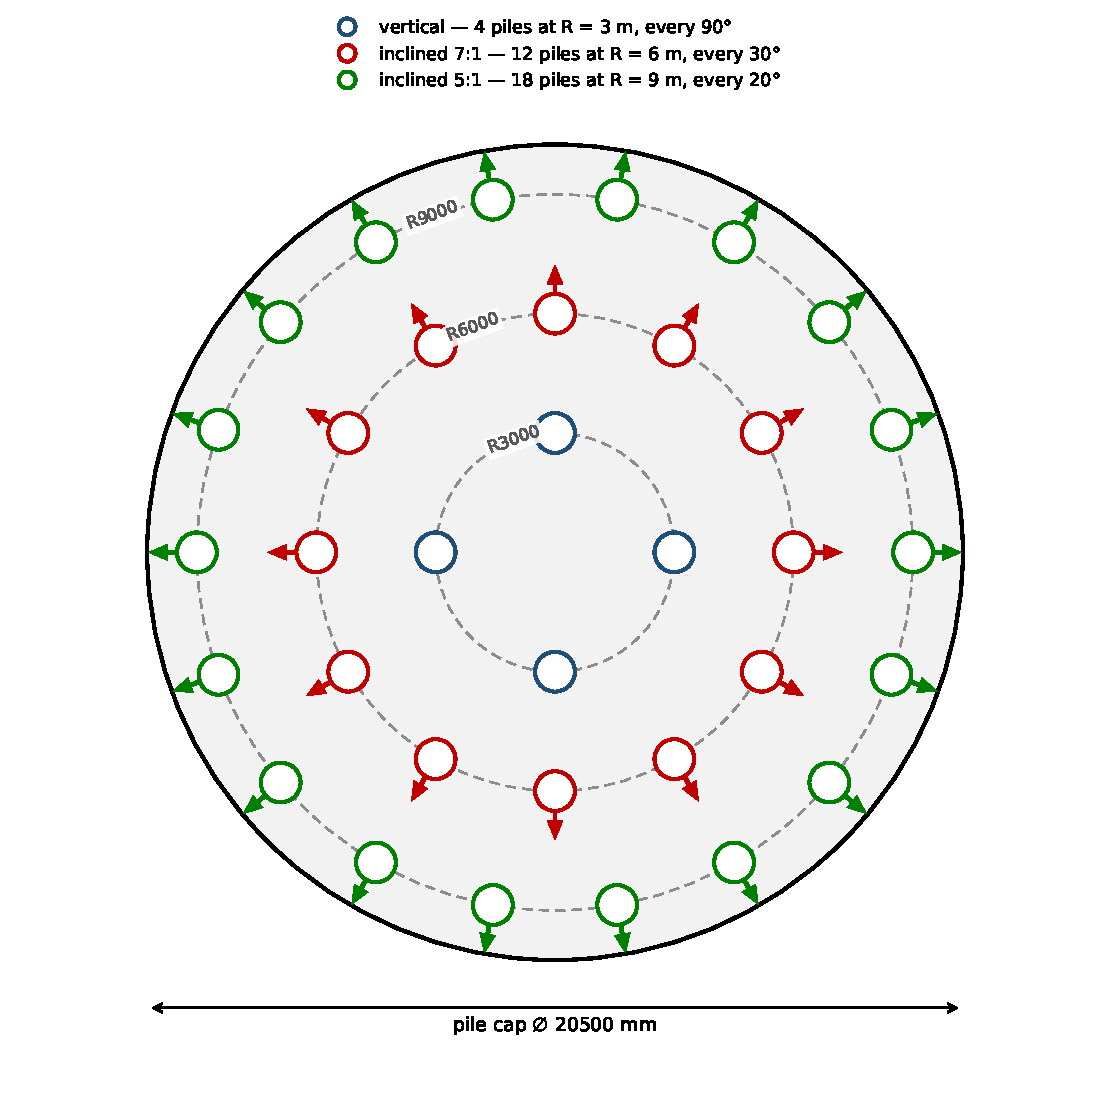
\includegraphics[width=0.72\linewidth]{fig01_pile_layout}
\caption{Pile layout of the T18 foundation, redrawn from the setting-out sheet \emph{D1000 PHC pile coordinate}: 34 PHC D1000 piles on three concentric rings of radius 3.0, 6.0 and 9.0~m, carrying 4, 12 and 18 piles respectively. Arrows give the direction of inclination; the inner ring is vertical, the middle ring is inclined 7:1 and the outer ring 5:1. The cap is 20.5~m in diameter}
\label{fig:layout}
\end{figure}

\begin{table}[htbp]
\centering
\caption{Foundation geometry and pile section properties, all read from the design drawings. The section properties enter the absolute frequency of Section~\ref{sec:criterion} and the stiffness comparison of Section~\ref{sec:stiffness}; they do not enter the criterion itself.}
\label{tab:geometry}
\begin{tabularx}{\linewidth}{@{}lL@{}}
\toprule
Cap & 20.5~m diameter, 4~m thick; soffit $+5.435$, top $+9.435$ \\
Inner ring & $R = 3.0$~m, 4 piles at 90\degr, vertical \\
Middle ring & $R = 6.0$~m, 12 piles at 30\degr, inclined 7:1 (8.1\degr{} from vertical) \\
Outer ring & $R = 9.0$~m, 18 piles at 20\degr, inclined 5:1 (11.3\degr{} from vertical) \\
Pile & prestressed high-strength concrete, 1.0~m outside diameter, 46~m long; toe at $\approx -40.5$ \\
Free length in water & 12.34~m (cap soffit $+5.435$ to seabed $-6.900$) \\
Wall thickness & 130~mm $\rightarrow$ $A = 0.3553$~m$^2$, $I = 0.03437$~m$^4$ \\
Elastic modulus & 40~GPa $\rightarrow$ $EA = 1.42\times10^{10}$~N, $EI = 1.37\times10^{9}$~N\,m$^2$ \\
\bottomrule
\end{tabularx}
\end{table}

Two lengths determine the dynamic behaviour of the ground beneath the foundation. The pile is unsupported over 12.34~m of water, and the first 13.4~m
below the seabed is very soft fat clay with SPT $N$ never exceeding 2, in which
it receives almost no lateral restraint. Together these place the whole flexible part of each pile in its upper third. The competent strata below --- very stiff lean clay from 16.0~m, medium
dense clayey sand to 30.5~m and very stiff fat clay beneath that --- act only
over the lower half.

This accounts for the fundamental frequency of this foundation falling near 1~Hz rather than in the range expected of a cap bearing on firm ground. The profile and the SPT record are reproduced in
Figure~\ref{fig:section}.

\begin{figure}[htbp]
\centering
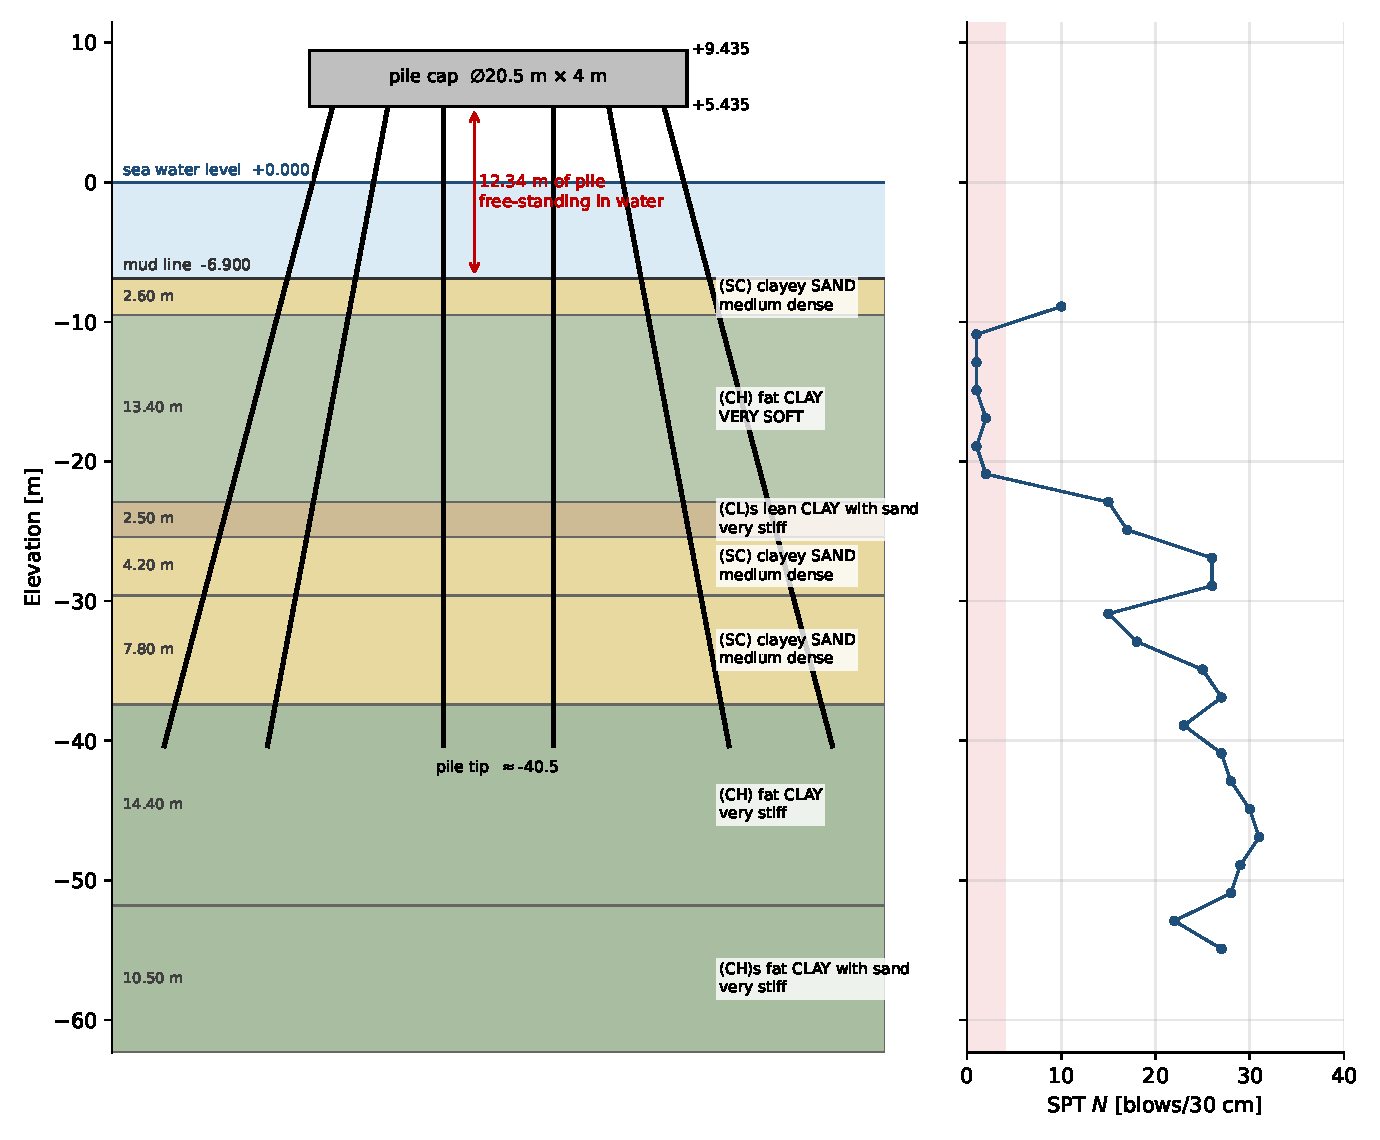
\includegraphics[width=0.85\linewidth]{fig02_foundation_section}
\caption{Foundation section and the soil profile at borehole DH9, with the SPT record alongside. Elevations are in metres. Each pile stands free in water over 12.34~m between the cap soffit at $+5.435$ and the seabed at $-6.900$. The fat clay immediately below the seabed is very soft, with $N \leq 2$ over 13.4~m}
\label{fig:section}
\end{figure}

\subsection{Instrumentation and measurement campaigns}
\label{sec:records}

Two ambient vibration campaigns were recorded on the top surface of the cap:
campaign 1 before the tower was erected and campaign 2 after. Each comprises
several setups differing in sensor position and measurement direction, seven in
total, with three to six accelerometers sampled at 1651~Hz for between 9 and 26
minutes. The instrumented area is a square frame of $5 \times 5$~m with sensors
at the four corners and at the centre and, in campaign 2, a sixth channel two
metres above the centre on the tower itself. Figure~\ref{fig:sensors} shows the
arrangement. The position of the frame on the 20.5~m cap is not documented, and it is drawn concentric on the inference that the sixth channel, being mounted on the tower, lies close to the cap centre.

\begin{figure}[htbp]
\centering
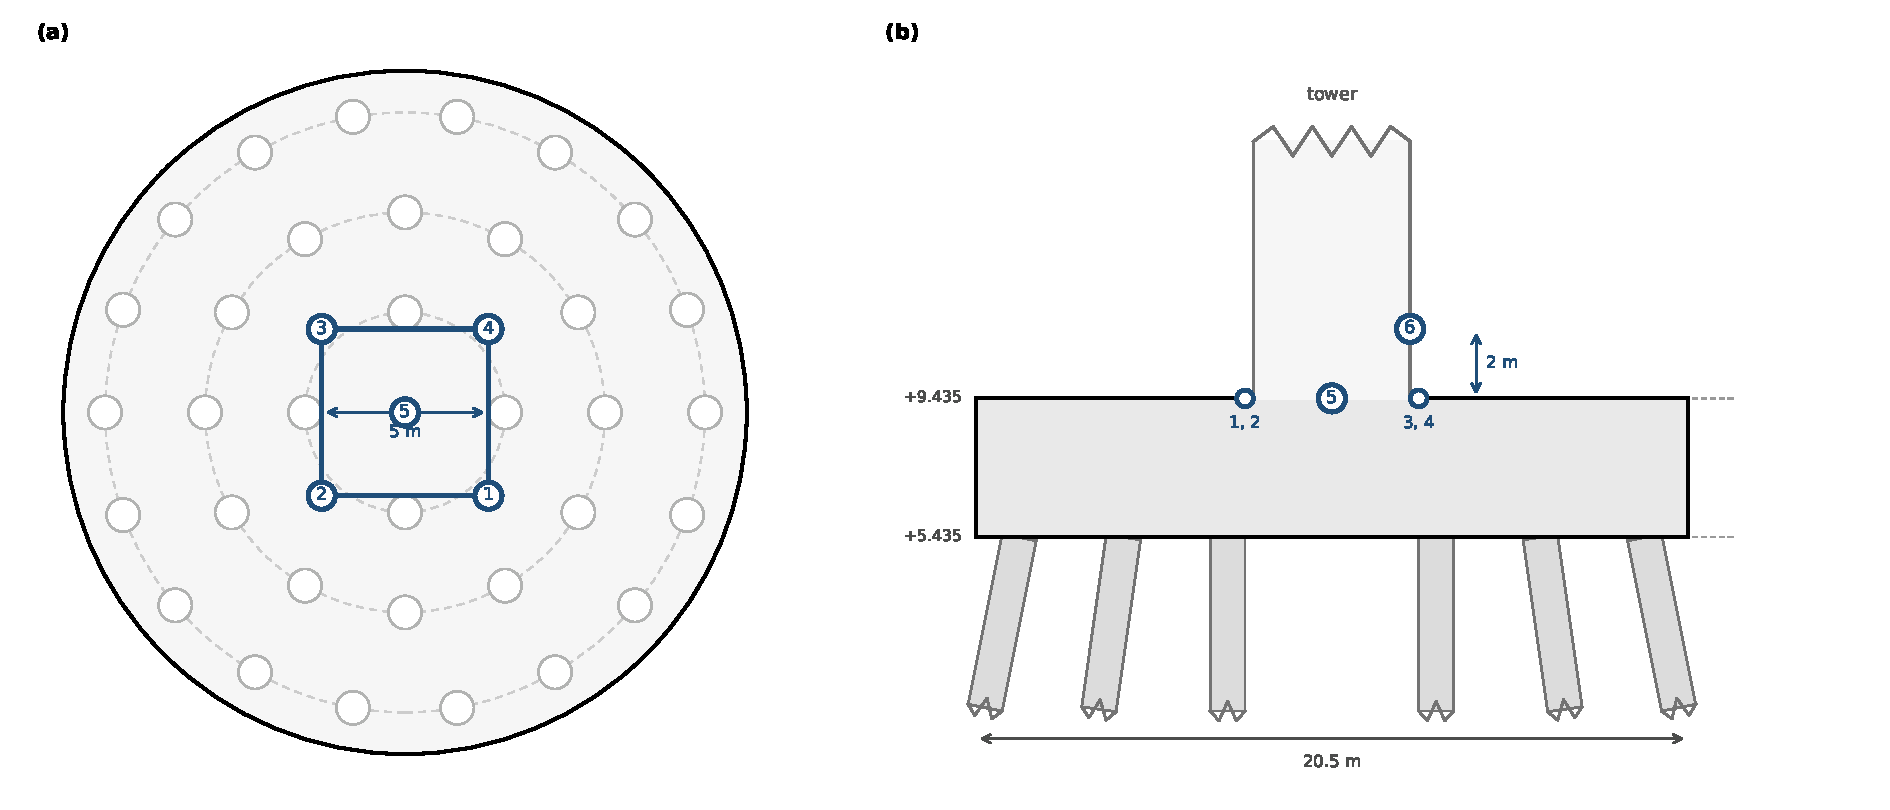
\includegraphics[width=0.98\linewidth]{fig03_sensor_layout}
\caption{The instrumented frame. (a) Plan of the $5 \times 5$~m frame on the 20.5~m cap, with channels 1 to 4 at the corners and channel 5 at the centre. (b) Elevation, showing the sixth channel of campaign 2, which is mounted on the tower two metres above the cap surface and so cannot be placed in the plan. Only the six piles cut by a diametral section are drawn, and both they and the tower are shown broken off rather than at full length. The vertical setups measure $Z$ on every channel; the lateral setups measure horizontally on channels 1, 2, 3 and 5 and vertically on channel 4. The position of the frame on the cap is not documented, and it is drawn concentric on the inference that channel 6, being on the tower, lies close to the cap centre}
\label{fig:sensors}
\end{figure}

\begin{table}[htbp]
\centering
\caption{Measurement setups and raw-record statistics. \emph{Peak}/$\sigma$ is
the largest absolute sample of any channel divided by that channel's standard
deviation; \emph{RMS drift} the ratio of largest to smallest channel RMS over
ten equal segments; \emph{spread} the ratio of the largest to the smallest
channel standard deviation within a setup.}
\label{tab:records}
\begin{tabular}{@{}llrrrrrrrr@{}}
\toprule
Camp. & Setup & Ch. & Samples & Min & Peak/$\sigma$ & Kurtosis & $>8\sigma$ & RMS drift & Spread \\
\midrule
1 & Vertical       & 5 & 2\,535\,936 & 25.6 & 133 & 562  & 2238 & 3.2 & 6.1 \\
1 & Lateral 1      & 5 & 1\,523\,873 & 15.4 & 25  & 54   & 3131 & 12.9 & 47.0 \\
1 & Lateral 2      & 5 & 1\,385\,189 & 14.0 & 50  & 1812 & 1063 & \textbf{112} & 9.2 \\
1 & Three-channel  & 3 & 1\,545\,336 & 15.6 & 10  & 4    & 9    & 1.5 & 33.7 \\
2 & Lateral        & 6 & \phantom{0}906\,399 & \phantom{0}9.2 & \textbf{139} & \textbf{3883} & 724 & 4.7 & 11.5 \\
2 & Vertical d1    & 6 & 1\,875\,536 & 18.9 & 69  & 95   & 695  & 4.4 & 4.1 \\
2 & Vertical d2ke  & 6 & 2\,260\,219 & 22.8 & 67  & 88   & \textbf{2564} & 4.3 & 4.2 \\
\bottomrule
\end{tabular}
\end{table}

The excitation is not the process the identification method assumes, and the
departure is larger in campaign 1 than in campaign 2. Figure~\ref{fig:quality} shows one campaign 2 record. A single event in it reaches 139 standard deviations of its channel and carries the kurtosis of a nine-minute record to 3883, and the running RMS shows that the event is confined to one channel. Of the signal energy, 78.6\,\% lies between 50 and 200~Hz and 0.7\,\% in the structural band from 0.2 to 5~Hz. Table~\ref{tab:records} shows that campaign 1 is worse on two counts. In the
lateral 2 setup the segment RMS varies by a factor of 112 within one record. In
the lateral 1 setup one channel is 47 times weaker than another in the same
setup, so that setup carries fewer usable channels than its nominal count suggests.
Only the three-channel setup of campaign 1 approaches stationary broadband
behaviour, with a peak of $10\sigma$ and a kurtosis of 4.

\begin{figure}[htbp]
\centering
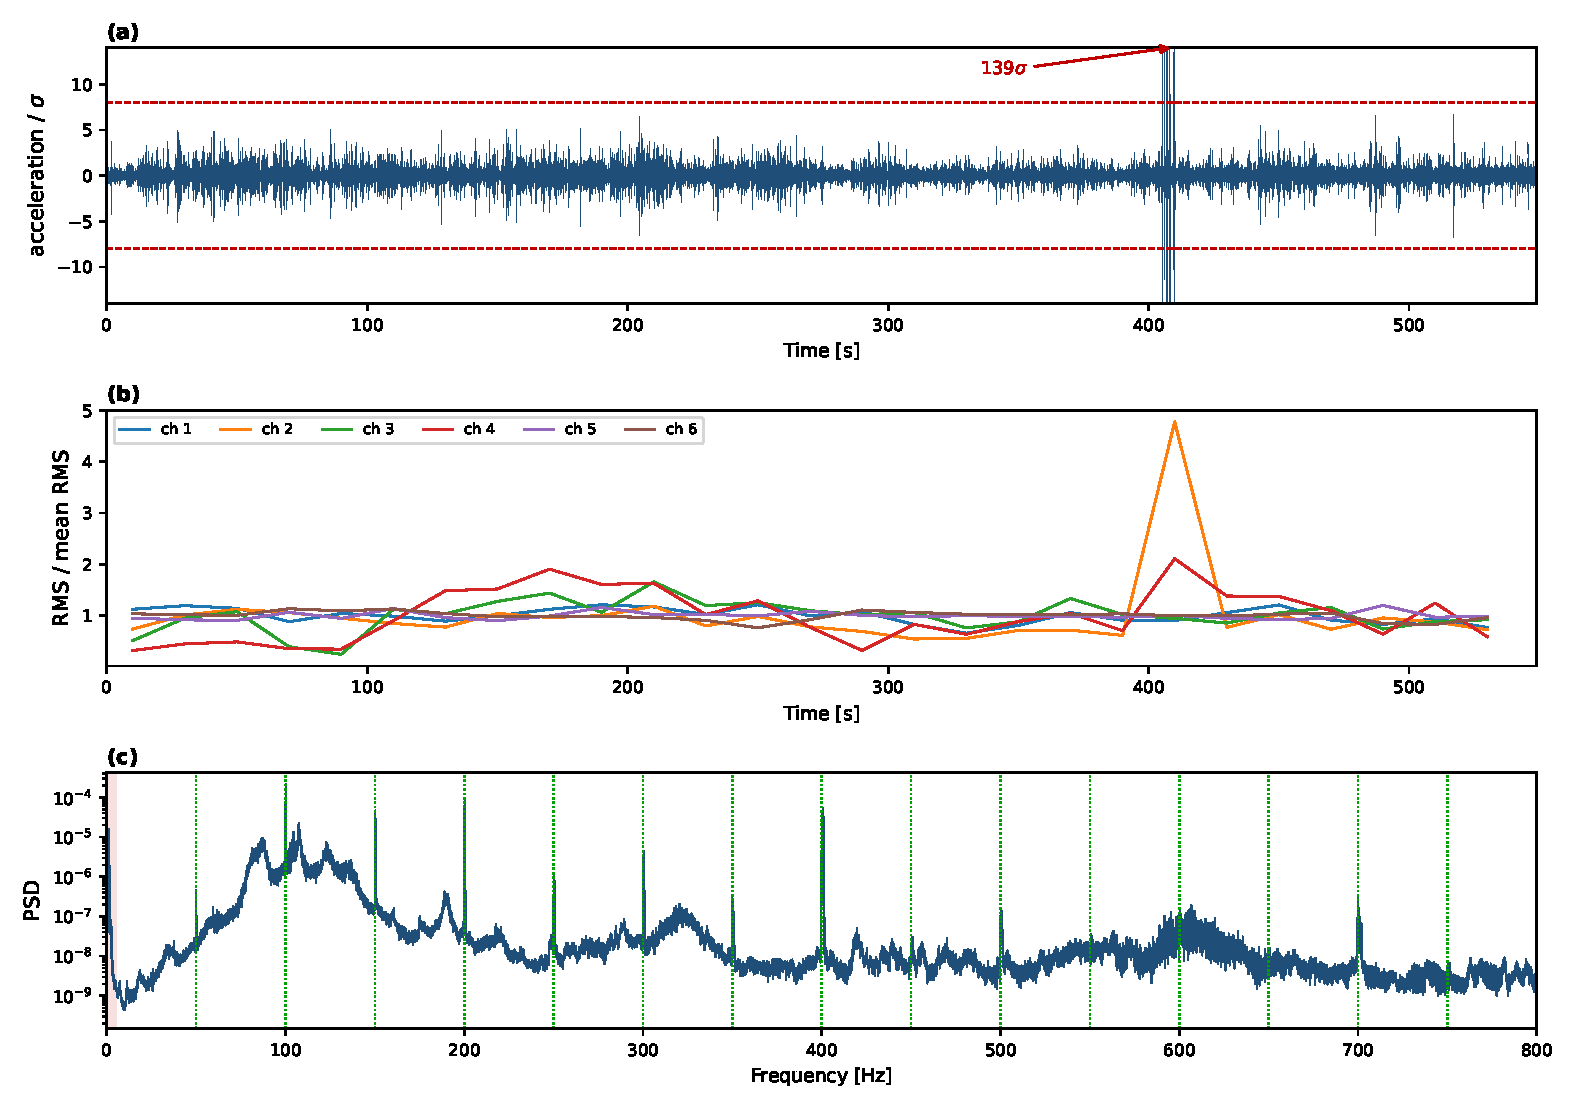
\includegraphics[width=0.95\linewidth]{fig04_record_quality}
\caption{One record of campaign 2 in three views. (a) The full time history of the channel with the largest peak-to-standard-deviation ratio, in units of that channel's standard deviation and with the $\pm 8\sigma$ band marked. The vertical scale is clipped at $\pm 14\sigma$ so that the ambient level remains legible; the single event at 408~s reaches $139\sigma$, carries the record kurtosis to 3883, and is marked by the arrow. (b) The running RMS of every channel over 20~s windows, normalised by its own mean; the event of panel (a) is confined to one channel. (c) The channel-averaged spectrum, with multiples of 50~Hz dotted; the band from 50 to 200~Hz carries 78.6\,\% of the energy and the shaded structural band from 0.2 to 5~Hz carries 0.7\,\%}
\label{fig:quality}
\end{figure}

Two consequences follow. Damping ratios are reported where the identification produces them, because the
stabilisation criterion uses them, but they are not interpreted. Subspace
damping estimates under impulsive, non-stationary excitation are biased by an
unknown amount, and field studies of offshore support structures report damping
that varies with load level and operating state \cite{noren2021}. Frequency estimates, in addition, carry more uncertainty than the scatter within a stabilisation cluster suggests, and for that reason Section~\ref{sec:classify} does not rest on frequency agreement between setups.

% =====================================================================
\section{A geometric criterion for sway and rocking}
\label{sec:model}

The derivation that follows uses no measurement. It starts from the equation of motion of a rigid body supported on axial springs, assembles the lateral and rotational stiffness of an inclined pile group, and shows that the axial pile stiffness cancels from the ratio of the two natural frequencies. Because the result is fixed before any record is examined, the comparison in Section~\ref{sec:mechanism} is a test and not a fit.

\subsection{Idealisation and the stiffness of an inclined pile group}
\label{sec:idealisation}

The cap is treated as a rigid body and each pile as a spring acting along its
own axis, together with a transverse spring representing its bending. The
idealisation is appropriate here because the cap is 4~m thick over a 20.5~m span
while the piles are 1.0~m in diameter over 46~m: the cap is orders of magnitude
stiffer in the relevant deformation than the elements supporting it. Under this idealisation the foundation has the two degrees of freedom that matter: a translation of the cap, and a rotation about a horizontal axis through its centre. Which mechanism governs the lowest mode is then a question about two stiffnesses.

Resolving the axial stiffness of a single pile onto those degrees of freedom
introduces the angle of inclination twice, in two different ways, and this is the origin of the result. Consider a pile at radius $r$ and azimuth $\theta$,
inclined outward at an angle $\alpha$ from vertical, so that its axis has unit
vector $(\sin\alpha\cos\theta,\ \sin\alpha\sin\theta,\ \cos\alpha)$. Under a
horizontal translation $u$ of the cap, the axial extension of that pile is the
projection $u\sin\alpha\cos\theta$: only the component of cap displacement lying
along the pile axis stretches it, so the contribution to lateral stiffness
carries $\sin^2\alpha$. Under a rotation $\varphi$ of the cap about a horizontal
axis, the pile head is displaced vertically by $\varphi\, r\cos\theta$, of which
the component along the pile axis is $\varphi\, r\cos\theta\cos\alpha$, so the
contribution to rotational stiffness carries $r^2\cos^2\alpha$. Summing over the
group and adding the bending term,
%
\begin{align}
k_{\mathrm{lat}} &= k_{\mathrm{ax}} \sum_i \sin^2\alpha_i
   + \frac{12EI}{L_{\mathrm{eff}}^{3}} \sum_i \cos^2\alpha_i , \label{eq:klat}\\
k_{\theta} &= k_{\mathrm{ax}} \sum_i r_i^2 \cos^2\alpha_i , \label{eq:ktheta}
\end{align}
%
in which $k_{\mathrm{ax}}$ is the axial stiffness of one pile and
$L_{\mathrm{eff}}$ its effective fixity length.

Figure~\ref{fig:mechanisms} shows the two mechanisms and the sense in which each
loads the piles. Two features of the formulation matter.
First, both mechanisms load the piles axially, and in both the axial
displacement field is antisymmetric in azimuth, proportional to $\cos\theta$ in
each case; this becomes important when pile-group interaction is considered in
Section~\ref{sec:criterion}. Second, the formulation already marks a boundary of
the result: a group of vertical piles has $\sin\alpha = 0$ and therefore no axial contribution to lateral stiffness. For such a group, sway is
resisted by pile bending alone, the two stiffnesses are no longer proportional
to a common quantity, and the criterion derived next does not apply.

\begin{figure}[htbp]
\centering
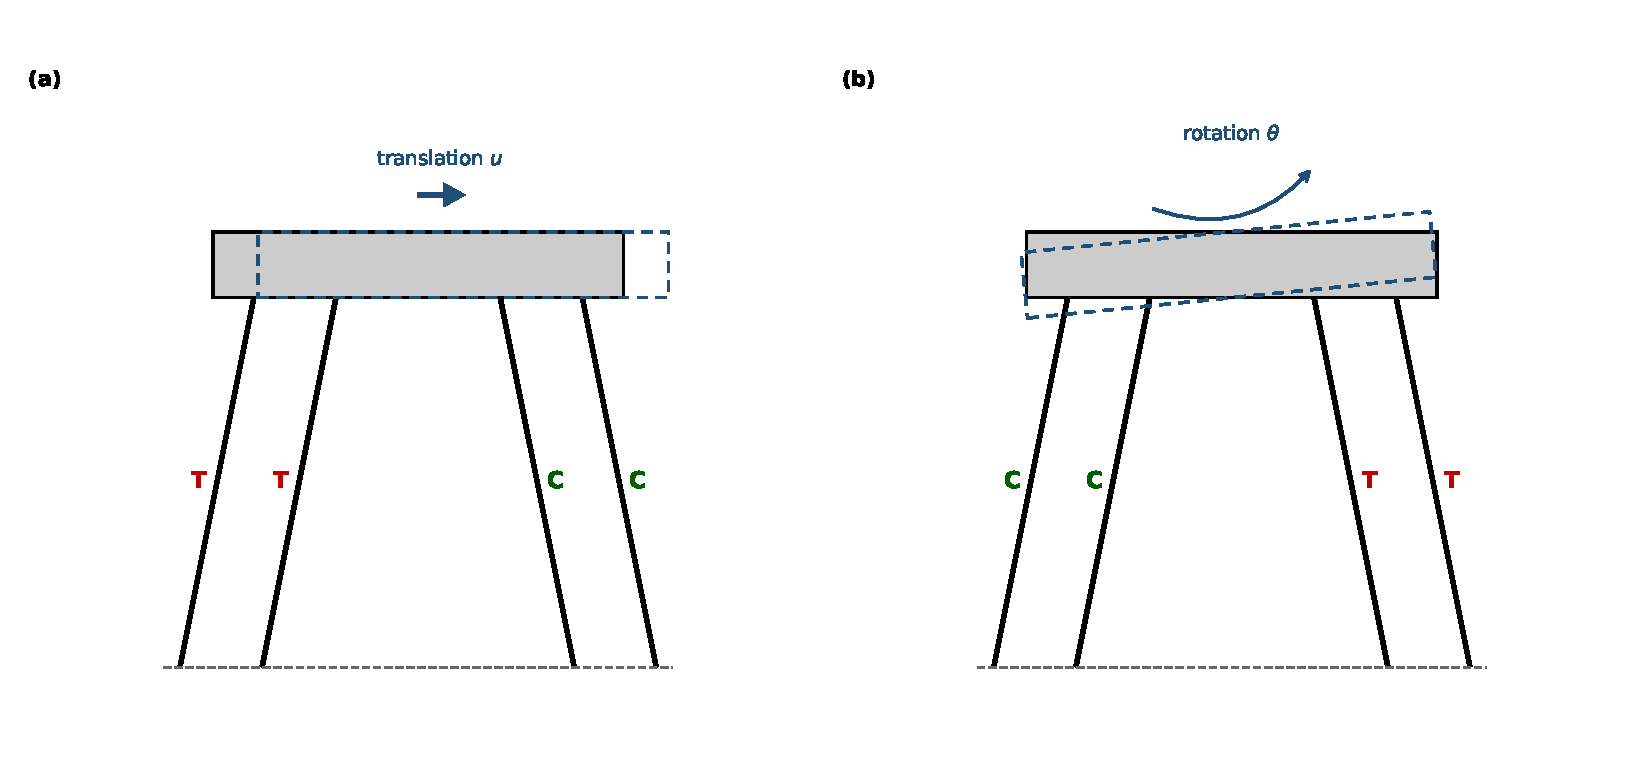
\includegraphics[width=0.95\linewidth]{fig05_mechanisms}
\caption{The two mechanisms available to a rigid cap on an inclined pile group. (a) Sway, resisted by the axial stiffness of the inclined piles together with pile bending. (b) Rocking, resisted by the same axial stiffness acting on the lever arms. Dashed outlines give the displaced position; C marks a pile in compression and T a pile in tension}
\label{fig:mechanisms}
\end{figure}

\subsection{Cancellation of the soil stiffness}
\label{sec:criterion}

Both stiffnesses in \eqref{eq:klat} and \eqref{eq:ktheta} are proportional to
the same axial pile stiffness. Setting the bending term aside for the moment,
$k_{\mathrm{ax}}$ cancels when the ratio of the corresponding natural
frequencies is formed:
%
\begin{equation}
\frac{f_{\mathrm{rock}}}{f_{\mathrm{sway}}}
= \sqrt{\frac{k_\theta / J}{k_{\mathrm{lat}} / M}}
= \sqrt{\frac{\sum r_i^2\cos^2\alpha_i \big/ J}{\sum \sin^2\alpha_i \big/ M}} ,
\label{eq:ratio}
\end{equation}
%
in which $J$ is the mass moment of inertia of the foundation about the rotation
axis and $M$ its mass. Nothing on the right-hand side refers to the soil, to the
pile section or to the pile material. For a group in which all piles share one
angle of inclination the expression simplifies further. Writing $\sum r^2 = n\,
r_{\mathrm{rms}}^2$ and $\sum \sin^2\alpha = n \sin^2\alpha$, and
$k_g = \sqrt{J/M}$ for the radius of gyration of the mass,
%
\begin{equation}
\frac{f_{\mathrm{rock}}}{f_{\mathrm{sway}}}
= \frac{r_{\mathrm{rms}}}{k_g}\,\cot\alpha ,
\label{eq:dimensionless}
\end{equation}
%
two dimensionless numbers: the reach of the pile ring relative to the inertia of the mass it supports, and the inclination.

This form makes the range of validity explicit. The two mechanisms coincide when
$\tan\alpha = r_{\mathrm{rms}}/k_g$. For a cap whose piles reach beyond its
radius of gyration, as any practical group does, that angle lies above
45\degr; for the foundation studied here it is 52\degr. Inclinations used in construction are
an order of magnitude shallower, between 12:1 and 4:1, or 4.8\degr{} to
14.0\degr, so the ratio does not fall below about five for any practical inclined group, irrespective of the soil. Figure~\ref{fig:criterion} shows the relation over the
practical range for several values of $r_{\mathrm{rms}}/k_g$. A single
low-frequency band identified on such a foundation can only be sway.

\begin{figure}[htbp]
\centering
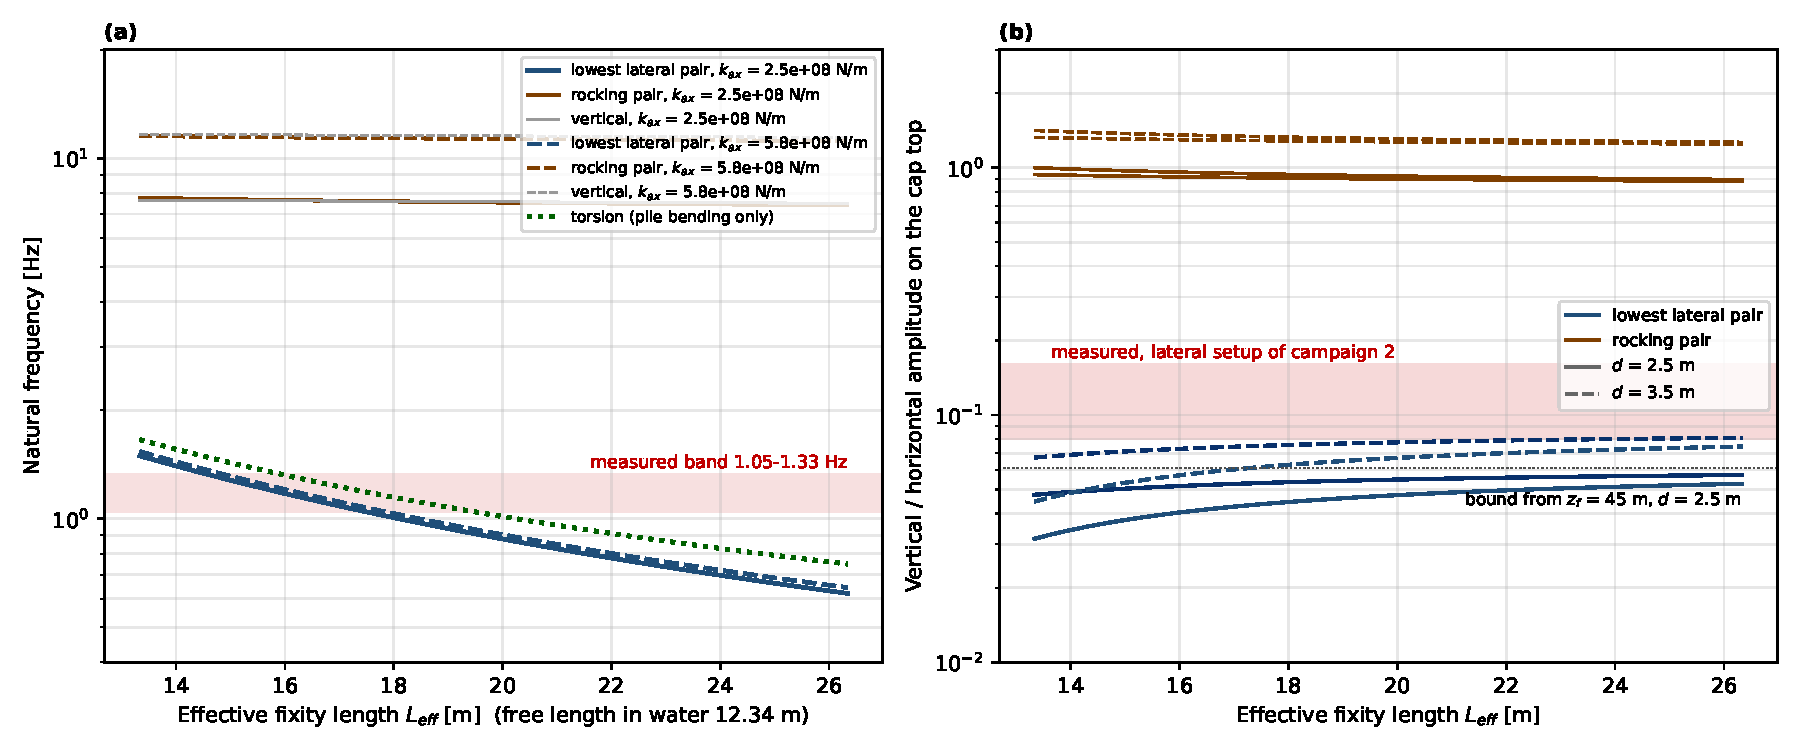
\includegraphics[width=0.8\linewidth]{fig06_criterion}
\caption{The criterion \eqref{eq:dimensionless} in dimensionless form, for several values of $r_{\mathrm{rms}}/k_g$. The shaded band covers the inclinations used in construction, 12:1 to 4:1. The horizontal line is $f_{\mathrm{rock}} = f_{\mathrm{sway}}$, reached only at the marked angle $\alpha_{\mathrm{crit}}$, which lies far outside that band}
\label{fig:criterion}
\end{figure}

One mechanism could break the cancellation. Pile--soil--pile interaction reduces the stiffness of a group below the sum of its isolated piles, and it would not cancel if the two mechanisms mobilised the soil differently. It is therefore computed here rather than assumed away. Elastic axial interaction factors
\cite{randolph1979}, $\alpha_{ij} = \ln(r_m/s_{ij}) / \ln(r_m/r_0)$ with
$r_m = 2.5\,L_{\mathrm{emb}}(1-\nu)$, are assembled over the 34 actual pile
positions. For a rigid cap, a mechanism whose unit axial displacement vector is
$\mathbf{v}$ then has group efficiency
$\eta = (\mathbf{v}^{\mathsf T}\mathbf{A}^{-1}\mathbf{v})/(\mathbf{v}^{\mathsf T}\mathbf{v})$.
The effect very nearly cancels as well, for the reason identified in
Section~\ref{sec:idealisation}: both mechanisms produce axial displacement
fields proportional to $\cos\theta$, so in both the interactions between piles
on opposite sides of the cap oppose one another. The efficiencies are 0.447 for
sway and 0.399 for rocking, against 0.075 for uniform settlement, in which all
piles move in the same sense and the interactions accumulate instead. The ratio
is corrected by $\sqrt{0.399/0.447} = 0.945$.

Table~\ref{tab:sums} collects the geometric sums and the resulting values for
this foundation. The ratio is 7.69 with the group treated as isolated piles and
7.26 with interaction included, and the bending term, when restored, moves it
between 6.15 and 7.48 over a tenfold range of assumed axial stiffness. Rocking lies approximately seven times above sway on this foundation, and no plausible variation of the assumptions brings it within a factor of five.

\begin{table}[htbp]
\centering
\caption{Geometric sums and the resulting frequency ratio for the T18 group.}
\label{tab:sums}
\begin{tabular}{@{}lr@{}}
\toprule
$\sum r^2\cos^2\alpha$ & 1861.3~m$^2$ \\
$\sum \sin^2\alpha$ & 0.9323 \\
$\sum \cos^2\alpha$ & 33.07 \\
$M$ (cap, piles and added water) & $5.03\times10^{6}$~kg \\
$J$ & $1.698\times10^{8}$~kg\,m$^2$ \\
$r_{\mathrm{rms}}$ , $k_g$ & 7.53~m , 5.81~m \\
Group efficiency: sway / rocking / uniform & 0.447 / 0.399 / 0.075 \\
$f_{\mathrm{rock}}/f_{\mathrm{sway}}$, isolated piles & \textbf{7.69} \\
$f_{\mathrm{rock}}/f_{\mathrm{sway}}$, with group interaction & \textbf{7.26} \\
Inclination at which the mechanisms coincide & 52\degr \\
\bottomrule
\end{tabular}
\end{table}

The cancellation is a first-order result under the idealisation of
Section~\ref{sec:idealisation}, not a universal property of inclined pile groups,
and the limits belong with it. It assumes a rigid cap, small motion, a single
effective axial stiffness entering both mechanisms, and static rather than
frequency-dependent pile stiffness. Full impedance analyses of inclined pile
groups show that group stiffnesses depend on excitation frequency, on the
soil--pile stiffness ratio, on spacing and on direction of inclination, and that
horizontal--rocking cross-coupling can be significant and can change sign with
configuration \cite{padron2010}. The ordering survives those complications; the numerical value does not.
The two mechanisms are separated by a factor of seven under the present
idealisation, whereas the corrections a full impedance treatment would
introduce are of order tens of per cent. The
criterion should be read as a screening test for which mechanism to expect, to
be set aside where a full impedance model is available.

The section does not give the absolute frequency. That depends on $k_{\mathrm{ax}}$, and therefore on the soil and on the effective fixity length, neither of which is known here to better than a factor of two; sweeping them spans 1.06 to 2.13~Hz, as Figure~\ref{fig:sensitivity} shows. The
model answers which mechanism governs, not at what frequency it appears.

\begin{figure}[htbp]
\centering
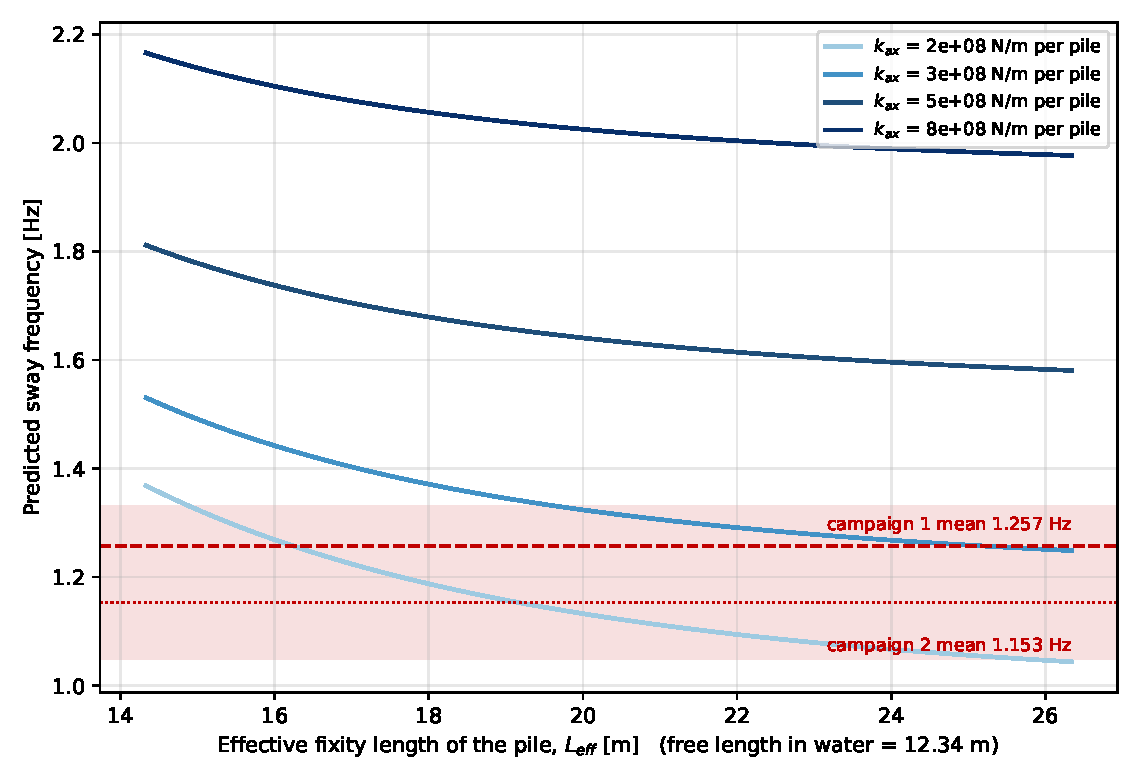
\includegraphics[width=0.8\linewidth]{fig07_sensitivity}
\caption{Sensitivity of the predicted sway frequency to the two governing assumptions, the effective fixity length $L_{\mathrm{eff}}$ and the axial pile stiffness $k_{\mathrm{ax}}$. The horizontal lines are the campaign means and the shaded strip the measured band, 1.05 to 1.33~Hz}
\label{fig:sensitivity}
\end{figure}

% =====================================================================
\section{Modal identification}
\label{sec:ident}

Identification supplies candidate poles; it does not supply modes.

\subsection{Identification procedure and acceptance criteria}
\label{sec:procedure}

Covariance-driven subspace identification assembles a block Toeplitz matrix of
output covariances up to lag $2i$ and recovers the state and output matrices
from its singular value decomposition \cite{peeters1999,overschee1996}. The
estimator therefore observes the record through a time window
$\tau = i\,\Delta t$, and this is a property of the construction rather than a
processing choice. A mode of period $T$ enters the covariances through their
oscillation and decay across that window; when $\tau \ll T$ the covariance
varies negligibly over the observed lags and carries nothing that distinguishes
the mode from a constant offset. The lowest frequency the estimator can resolve
is fixed, for a given configuration, before the data are consulted.

The processing chain follows from that requirement. Retaining the acquisition
rate of 1651~Hz with $i = 150$ gives $\tau = 0.091$~s, which is 9\,\% of one
period at 1~Hz and places any such mode outside the span of the estimator. The records are therefore decimated in two stages to 51.59~Hz with zero-phase
anti-alias filtering, then high-pass filtered at 0.3~Hz with a fourth-order
Butterworth. Identification uses $i = 120$ over model orders 2 to 80, which
gives $\tau = 2.33$~s, or 2.3 periods at 1~Hz. Poles are accepted into a cluster
when successive orders agree to within 1\,\% in frequency, 5\,\% in damping and
0.98 in modal assurance criterion, and a cluster is retained when it contains at
least eight poles. A frequency domain decomposition of the same records
\cite{brincker2001} provides an independent check.
Section~\ref{sec:classify} tests the resolution argument directly.

Three requirements are used as acceptance criteria. Each follows from the definition of a mode rather than from a convention of practice, each is stated as a property of the structure, and each can be evaluated on the raw records alone.

The first requirement is that a mode moves more than one measurement point. The mode shape is defined over the structure. If the observed shape has support
on one channel and noise elsewhere, then the motion is confined to a region
smaller than the sensor spacing, and the pole describes that region rather than
the structure the instrumentation was placed to characterise. The measure used is the effective channel count
$N_{\mathrm{eff}} = (\sum|\phi|^2)^2 / \sum|\phi|^4$, taken from the first
singular vector of the cross-power spectral density matrix. It equals the number of channels when the shape is spread evenly over them, and unity when one channel carries the entire response. The rejection threshold is established by simulation.
Synthetic records were generated at the same length and spectral resolution as
the measurements, once with a narrow-band signal on a single channel and once
with the same signal shared by all channels in a shape containing a nodal line.
The first case gives $N_{\mathrm{eff}} \le 1.00$ without exception. The second
gives $\ge 1.53$ for five channels and $\ge 1.74$ for six, in 95\,\% of trials. A threshold of $N_{\mathrm{eff}} = 1.25$ separates them with no overlap
in 400 trials per case. The quantity is the inverse participation ratio, familiar from studies of
vibrational localisation in disordered media \cite{bell1970,hodges1982}. No precedent was found for its use as an acceptance criterion in operational modal analysis, so it is defined explicitly here and justified by the simulations above rather than by citation. It is not a mass participation factor and should not be interpreted as one.

The second requirement is that a mode is the same for every observer. The eigenvalue depends on the mass, damping and stiffness of the structure, not
on which degrees of freedom are instrumented; moving the sensors changes which
components of the shape are observed and cannot change the eigenvalue. The
criterion requires the same pole in every setup of a campaign and, where the
measured degrees of freedom coincide, agreement of the shapes by the modal
assurance criterion.

The third requirement is that a mode dissipates at a rate materials permit. Free decay follows an envelope $e^{-\xi\omega t}$, so a mode falls to $1/e$ of
its amplitude in $1/(2\pi\xi)$ cycles. At $\xi = 0.01$\,\% that is about 1600
cycles; at $\xi = 0.007$\,\% and 100~Hz it is about 2300 cycles, or 23 seconds of sustained oscillation. A built structure under ambient excitation does not sustain free vibration for thousands of cycles, whereas a deterministic harmonic of constant frequency and amplitude
presents to a covariance-driven estimator as exactly such a pole, its apparent
damping reflecting estimator resolution rather than dissipation
\cite{mohanty2004,jacobsen2005}. The screening bound used here, $\xi = 0.1$\,\%, is adopted on that basis. Published field damping estimates for offshore support structures vary with load level and operating state \cite{noren2021}, so no field value is adopted. The bound coincides instead with the lowest damping that EN 1991-1-4 tabulates for any structural element, a logarithmic decrement of 0.006 for parallel cables, against 0.03 to 0.10 ($\xi \approx 0.5$ to 1.6\,\%) for reinforced concrete structures \cite{en1991}. It is used only to reject, and it lies two orders of magnitude below the values the admitted band returns.

\subsection{Classification of the identified poles}
\label{sec:classify}

Applied to these records, the procedure returns poles in three well-separated
regions. There is a group between 1.05 and 1.33~Hz and a set between 14 and
24~Hz. A third set, between 57 and 700~Hz, appears only under a configuration
that retains the acquisition rate. Table~\ref{tab:poles} lists the accepted poles of the first two
by setup. Figure~\ref{fig:stab} shows the stabilisation diagram of one setup and illustrates the difficulty: both the 1.2~Hz pole and the 18--20~Hz cluster
stabilise cleanly over the full range of model orders, so nothing in the
stabilisation behaviour distinguishes them.

\begin{figure}[htbp]
\centering
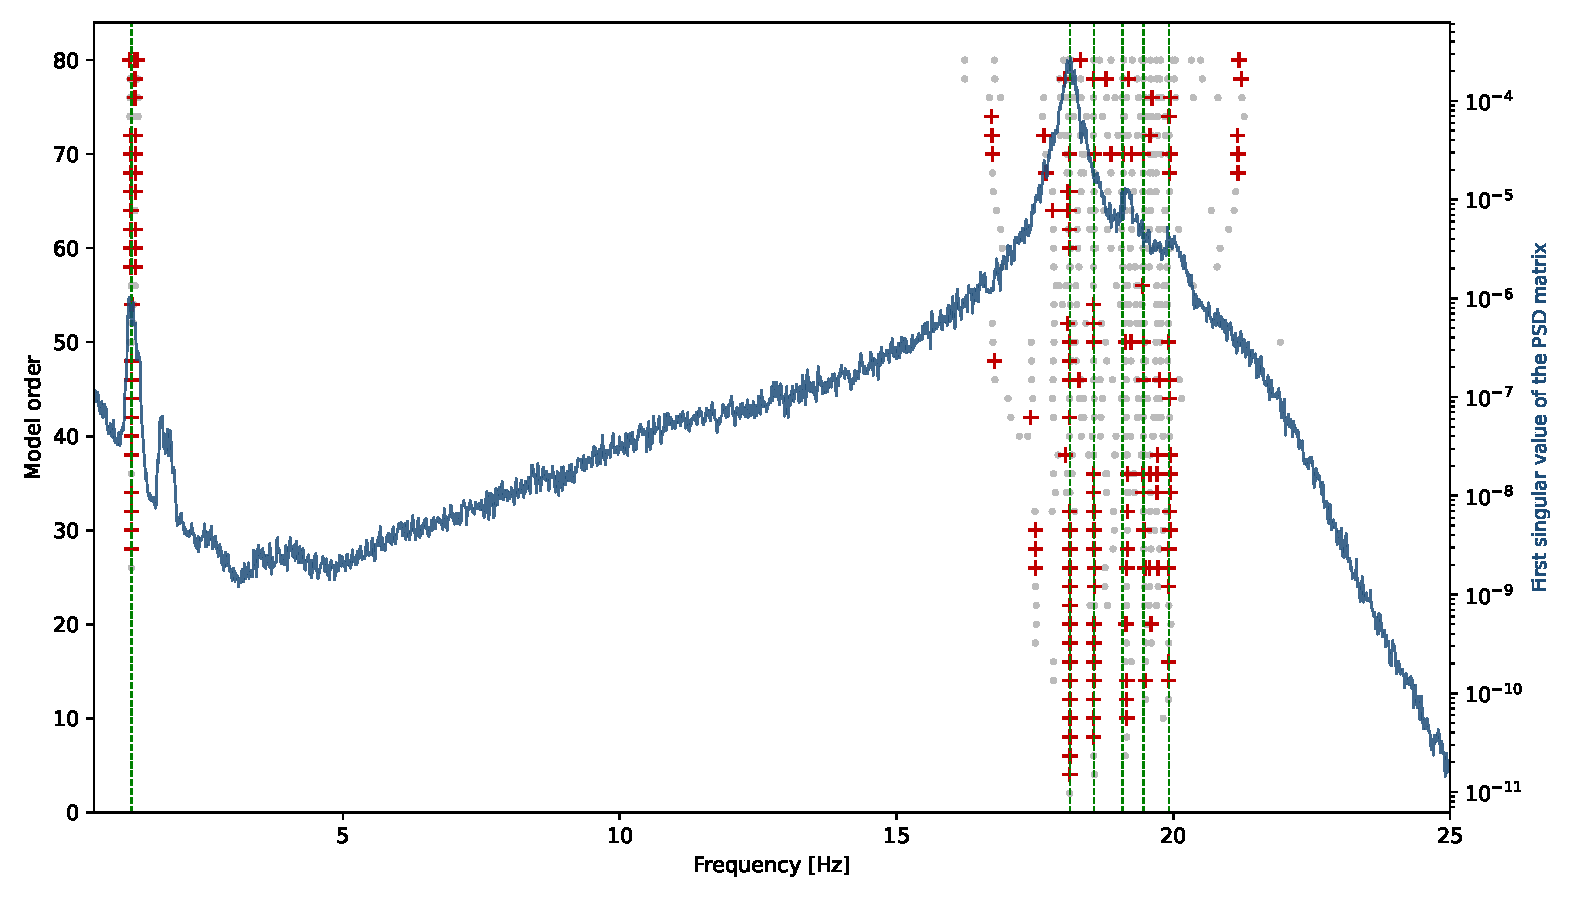
\includegraphics[width=0.95\linewidth]{fig08_stabilisation}
\caption{SSI-COV stabilisation diagram for the vertical setup of campaign 1, with the first singular value of the cross-power spectral density matrix overlaid. Both the 1.2~Hz pole and the 18--20~Hz cluster stabilise cleanly over the full range of model orders, so the stabilisation behaviour alone does not distinguish them}
\label{fig:stab}
\end{figure}

\begin{table}[htbp]
\centering
\caption{Accepted poles by setup; frequency in Hz with damping ratio in per cent
in parentheses.}
\label{tab:poles}
\begin{tabularx}{\linewidth}{@{}clLL@{}}
\toprule
Camp. & Setup & Low band & Higher band \\
\midrule
1 & Vertical & 1.173 (4.74) & 18.125 (0.70), 18.558 (0.68), 19.070 (0.58), 19.459 (0.59), 19.913 (1.30) \\
1 & Lateral 1 & 1.226 (3.43), 1.254 (2.77), 1.730 (5.49) & 21.912 (0.40), 22.742 (0.51), 23.745 (0.30) \\
1 & Lateral 2 & 1.322 (2.70) & 21.566 (5.95), 22.804 (1.25), 23.164 (0.59) \\
1 & Three-channel & 1.237 (3.01), 1.331 (4.39), 1.725 (5.35) & 14.432 (1.42), 14.990 (0.97) \\
2 & Lateral & 1.052 (2.68), 1.215 (1.93), 1.611 (2.42) & none accepted \\
2 & Vertical d1 & 1.147 (9.85) & 11.801, 13.866, 16.827, 17.081, 17.666, 18.947, 19.466, 19.682, 20.542 \\
2 & Vertical d2ke & 1.073 (1.25), 1.198 (2.35), 1.230 (2.48) & 2.295 (1.19) \\
\bottomrule
\end{tabularx}
\end{table}

Under the first requirement, Figure~\ref{fig:neff} gives the effective channel count for both bands in all seven setups. In the 13--24~Hz band five of the seven fall at or below 1.17,
four of them at exactly 1.00: one channel responds and the rest lie at noise
level, so there is no spatial pattern to interpret. In the 1.0--1.4~Hz band six
of the seven exceed the threshold, ranging from 1.55 to 5.00. The low-band values are not uniform, and uniformity is not to be expected, since a pattern containing a nodal line necessarily leaves channels near that line with small amplitude, which
lowers $N_{\mathrm{eff}}$ without implying locality. Two exceptions are reported rather than excluded. Lateral setup 2 of campaign 1
gives 1.00 in the low band as well; it is also the record with the strongest
impulsive content, its narrow-band kurtosis \cite{jacobsen2007} lying between 128 and 164. The
three-channel setup gives 0.60 of its channel count in both bands, which with
only three channels does not separate the two cases.

\begin{figure}[htbp]
\centering
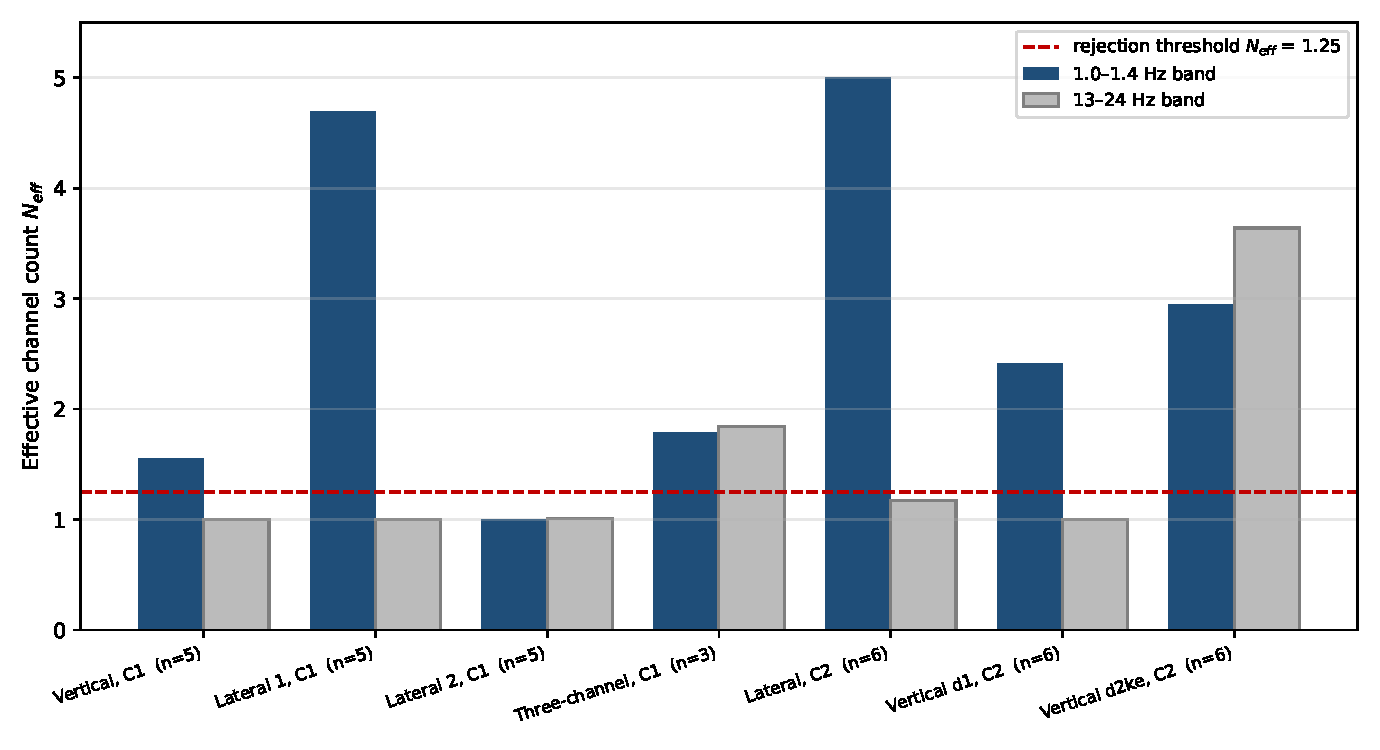
\includegraphics[width=0.85\linewidth]{fig09_participation}
\caption{Effective channel count $N_{\mathrm{eff}}$ by setup and band, against the rejection threshold of 1.25 established by simulation in Section~\ref{sec:procedure}. The number of channels in each setup is given in the axis label. A value of unity means that one channel carries the entire response}
\label{fig:neff}
\end{figure}

Under the second requirement, the low-band poles within a campaign spread by $\pm6.3$\,\% and $\pm7.7$\,\%. That is an order of magnitude more than the
scatter within a stabilisation cluster, so frequency agreement alone cannot
settle the question. The criterion is therefore applied to the shapes. In all three vertical setups of both campaigns, opposite corners of the
instrumented area move in antiphase, by 176\degr, 175\degr{} and 179\degr, about
a nodal line through the centre of that area. In the lateral setups all
horizontal channels move in phase and with similar amplitude. The two vertical
setups of campaign 2 instrument five points in common, and between their
corresponding clusters the modal assurance criterion is 0.967. The sixth channel
of each sits at a different point and is left out of that comparison.
Table~\ref{tab:phase} gives the phase relations and Figure~\ref{fig:shape} the
patterns. One further observation supports this interpretation. The single vertically oriented channel in the lateral setup is also the only channel there that is out of phase and of small amplitude, and it was not selected for that purpose.

By contrast the 14--24~Hz poles fail the same test. Within campaign 1
alone, three setups on the same cap in the same period return three disjoint
bands: 18.1 to 19.9~Hz, 21.6 to 23.7~Hz and 14.4 to 15.0~Hz. A natural frequency
is a property of the structure and cannot take three values at once.

One observation tells against the interpretation just given. If instead of matching corresponding clusters one
compares the first singular vector at the dominant low-band peak of each of
those two setups, the modal assurance criterion is 0.09, not 0.97. The peaks are
at 1.209 and 1.228~Hz, and the two setups are therefore dominated by different
members of the closely spaced group. The shapes of corresponding poles agree;
the dominant pole differs between setups. Both facts are consequences of the
group containing more than one mode, and Section~\ref{sec:mechanism} returns to
them.

\begin{figure}[htbp]
\centering
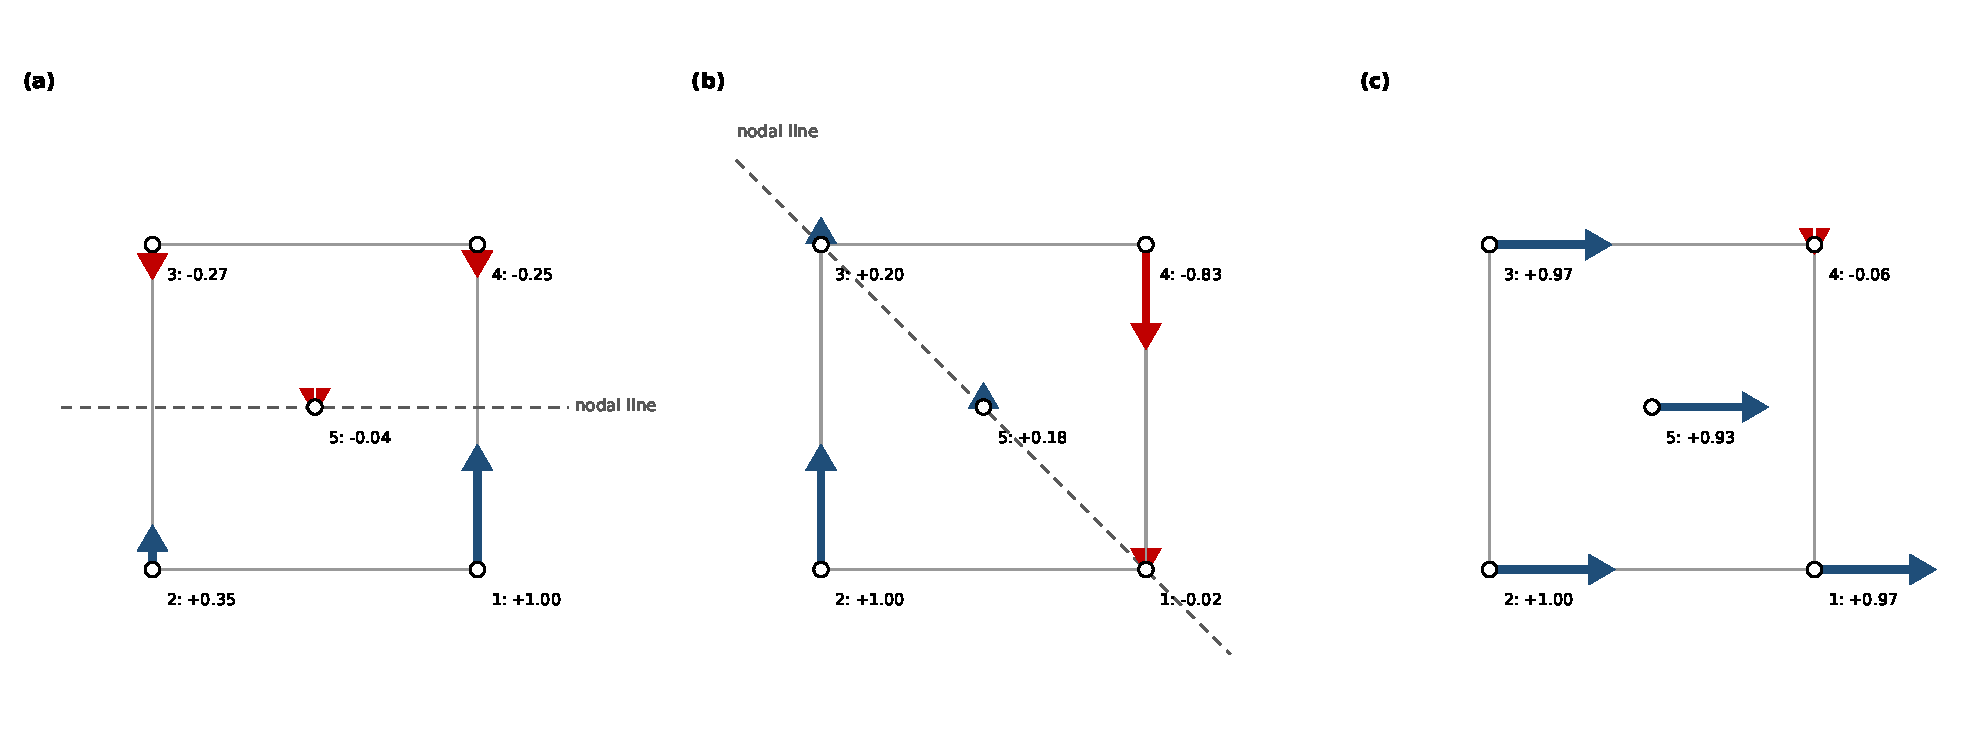
\includegraphics[width=0.98\linewidth]{fig11_mode_shape}
\caption{Measured deformation pattern of the 1.05--1.33~Hz band, taken from the first singular vector at the band peak. (a) Vertical setup of campaign 1. (b) Vertical setup d2ke of campaign 2. (c) Lateral setup of campaign 2. Signed amplitudes are given beside each node. The vertical setups show opposite corners in antiphase about a nodal line; the lateral setup shows the horizontal channels in phase, channel 4 being the only vertically oriented channel there}
\label{fig:shape}
\end{figure}

\begin{table}[htbp]
\centering
\caption{Phase between opposite corners of the instrumented frame at the
low-band peak, and amplitude at the centre relative to the mean of the corners.
In the lateral setup, channel 4 is the only vertically oriented channel, which
is why the 2--4 pair behaves unlike the 1--3 pair there.}
\label{tab:phase}
\begin{tabular}{@{}llrrrl@{}}
\toprule
Setup & Direction & Peak (Hz) & Node 1 vs 3 & Node 2 vs 4 & Centre / mean corner \\
\midrule
Vertical, campaign 1      & vertical   & 1.134 & $-179.1$\degr & $-173.3$\degr & 0.048 / 0.466 \\
Vertical d1, campaign 2   & vertical   & 1.209 & $+176.3$\degr & $+176.6$\degr & 0.424 / 0.517 \\
Vertical d2ke, campaign 2 & vertical   & 1.228 & $-142.7$\degr & $-175.2$\degr & 0.183 / 0.518 \\
Lateral, campaign 2       & horizontal & 1.203 & $-4.9$\degr   & $-143.3$\degr & 0.927 / 0.757 \\
\bottomrule
\end{tabular}
\end{table}

The third requirement needs the influence of the processing configuration settled first. Two processing choices govern what the identification can return, the covariance
window and the high-pass cut-off, and varying them together would not separate
their effects. One record was therefore processed under all four combinations,
Table~\ref{tab:config}. Configuration C removes the filter while keeping the
short window and still returns nothing below 5~Hz; configuration D lengthens the
window while keeping the filter and likewise returns nothing. Each constraint is
independently sufficient to suppress the admitted band, and only their joint
removal recovers it. The resolution limit of Section~\ref{sec:procedure} is
thereby established as a constraint in its own right and not a by-product of
filtering.

\begin{table}[htbp]
\centering
\caption{Factorial comparison of processing configurations, one record.}
\label{tab:config}
\begin{tabular}{@{}clllll@{}}
\toprule
Config. & Sampling rate & High-pass & $i$ & $\tau$ & Poles returned \\
\midrule
A & 1651~Hz & 5~Hz   & 150 & 0.091~s & 20, from 57.6 to 700.7~Hz; none below 5~Hz \\
C & 1651~Hz & 0.3~Hz & 150 & 0.091~s & 19, from 80.8 to 604.4~Hz; none below 5~Hz \\
D & 51.6~Hz & 5~Hz   & 120 & 2.33~s  & 6, from 6.8 to 20.6~Hz; none below 5~Hz \\
B & 51.6~Hz & 0.3~Hz & 120 & 2.33~s  & 3: 1.052, 1.215, 1.611~Hz \\
\bottomrule
\end{tabular}
\end{table}

Seven of the twenty poles returned by configuration A carry damping between
0.007\,\% and 0.042\,\%, which the third requirement alone rejects. Only
afterwards is the spectrum consulted, and it identifies them: the same seven lie
within 0.16\,\% of an exact multiple of 50~Hz, at 100.129, 150.239, 200.209,
250.171, 300.377, 400.537 and 700.666~Hz, and six of them survive into
configuration C. They are harmonics of the mains supply, which these records
carry at high level, as Figure~\ref{fig:harm} shows.

\begin{figure}[htbp]
\centering
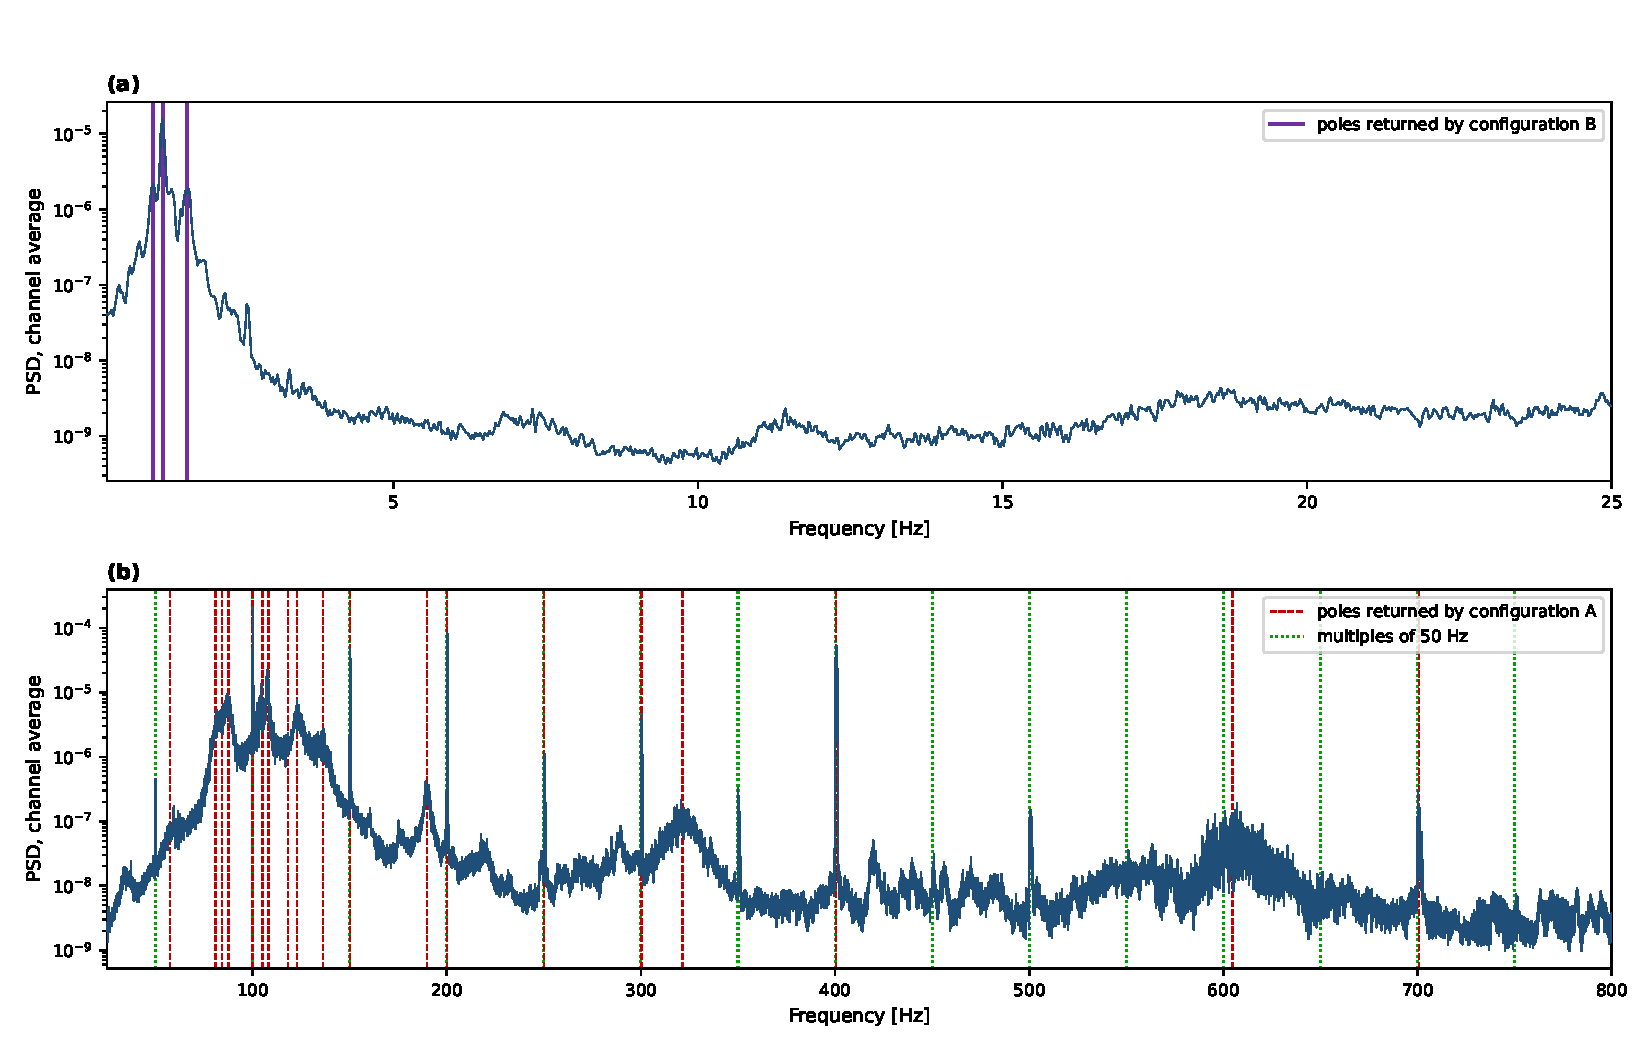
\includegraphics[width=0.95\linewidth]{fig10_configurations}
\caption{The same record seen by the two processing configurations of Table~\ref{tab:config}, over (a) the structural band from 0.3 to 25~Hz and (b) the band from 25 to 800~Hz from which configuration A draws its poles. Dotted lines mark multiples of 50~Hz}
\label{fig:harm}
\end{figure}

The region below the analysis band remains to be examined. The band searched begins at 0.5~Hz, which would exclude a tower mode: soft-stiff
design places the fundamental mode of a tower of this class between the $1P$ and
$3P$ rotor harmonics, near 0.3~Hz \cite{arany2017}. The records were therefore
reanalysed with a further decimation to 12.9~Hz and $i = 150$, a window of
11.6~s or 3.5 periods at 0.3~Hz, and searched from 0.18~Hz. No pole below 0.5~Hz
satisfies the criteria in any setup of either campaign. The only features there are peaks near 0.21~Hz in campaign 1 and 0.32~Hz in
campaign 2, each consistent between the setups of its own campaign. Their
periods are 4.7~s and 3.2~s, and they move upward between campaigns, which no
added-mass mechanism can produce. They are attributed to wave excitation under differing sea states.
Figure~\ref{fig:lowband} shows the search.

\begin{figure}[htbp]
\centering
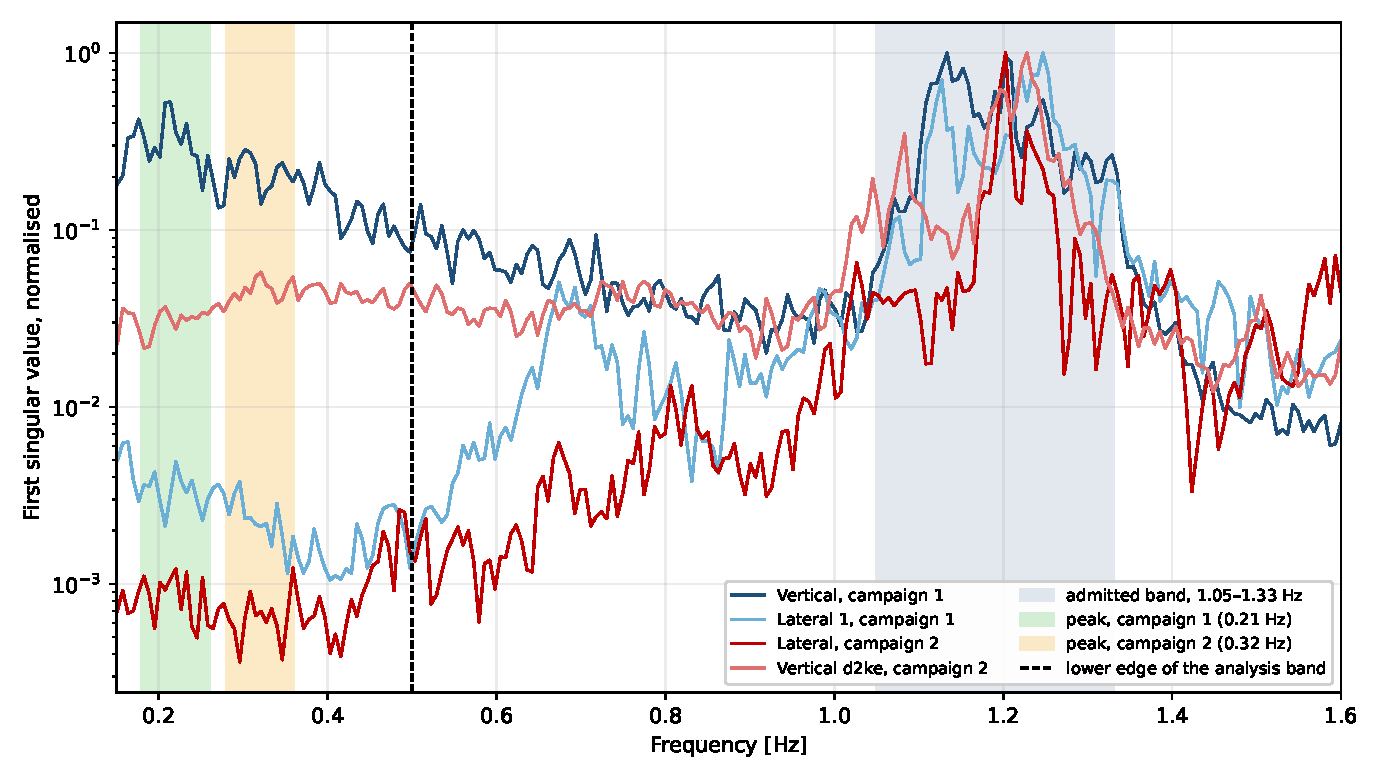
\includegraphics[width=0.85\linewidth]{fig12_low_band}
\caption{Search below the analysis band, with the records decimated to 12.9~Hz and a covariance window of 11.6~s. The only features below 0.5~Hz are the peaks marked at 0.21~Hz in campaign 1 and 0.32~Hz in campaign 2, which move upward between campaigns and are attributed to wave excitation}
\label{fig:lowband}
\end{figure}

Table~\ref{tab:classify} summarises the three requirements applied together. One band survives all three requirements;
the other two fail on grounds independent of each other and of the
identification settings.

\begin{table}[htbp]
\centering
\caption{Classification of the three groups of poles.}
\label{tab:classify}
\begin{tabularx}{\linewidth}{@{}lLLll@{}}
\toprule
Group & $N_{\mathrm{eff}}/n$ & Same in every setup & Damping & Verdict \\
\midrule
1.05--1.33~Hz & 0.31--0.94 in six of seven & yes; MAC 0.967 between corresponding clusters & 1.2--4.7\,\% & structural \\
14--24~Hz & 1.00 of 5 or 6 in five of seven & no; three bands in one campaign & 0.3--6\,\% & local to the sensor position \\
57--700~Hz & --- & --- & 0.007--0.042\,\% & mains harmonics \\
\bottomrule
\end{tabularx}
\end{table}

% =====================================================================
\section{Physical interpretation of the identified mode}
\label{sec:interp}

Sections~\ref{sec:model} and \ref{sec:ident} are independent of one another: the first uses only the geometry of the foundation, the second only the recorded motion. Combining them tests whether the mechanism the geometry requires is the mechanism the measurements show, and yields two quantities that neither line of evidence could give alone.

\subsection{Sway as the governing mechanism}
\label{sec:mechanism}

The geometry of Section~\ref{sec:model} places rocking 7.3 times above sway on this foundation, and the admitted band is the only low-frequency band in the records. The band is therefore sway. That conclusion is reached without any measurement, and it predicts what the measurements should show.

Sway of a rigid cap on inclined piles has a specific signature, and it is not a
pure translation. The cap translates horizontally under the lateral stiffness of
the group; but because the axial path through the piles is far stiffer than the
lateral one, the same motion also produces a small rotation about the cap
centre. The two components are seen by different sensors. A horizontally
oriented sensor sees the translation, which is common to every point of a rigid
cap, so all horizontal channels move in phase with comparable amplitude. A
vertically oriented sensor cannot see the translation at all, and records only
the rotation, which appears as opposite edges of the cap moving in antiphase
about a nodal line through its centre.

That is what Section~\ref{sec:classify} found, in every setup of both
campaigns: horizontal channels in phase, and vertical channels in antiphase
about a nodal line. Between corresponding clusters of the two vertical setups
the modal assurance criterion is 0.967, over the five points they instrument in
common. The prediction and the observation are drawn from disjoint information,
one from a setting-out drawing and the other from accelerometer records, and
their agreement is the central result of this paper.

Two qualifications apply. The nodal line
is located with respect to the instrumented frame, and the position of that
frame on the cap is not documented; the identification of its centre with the
cap centre rests on the inference set out in Section~\ref{sec:records}. The admitted band, moreover, is not a single mode: its spread within a campaign exceeds the
identification scatter by an order of magnitude, and the longest record resolves
three distinct poles within it, at 1.073, 1.198 and 1.230~Hz. The simplest explanation is a closely spaced orthogonal pair, resolved unequally by
setups having between three and six channels in one or two directions.
Section~\ref{sec:classify} supplies a second indication of the same effect: the two
vertical setups of campaign 2 are dominated by different members of the group,
so that their spectral peaks disagree even though their corresponding poles have
nearly identical shapes. Nothing in the mechanism argument depends on resolving
them.

\subsection{Equivalent axial pile stiffness}
\label{sec:stiffness}

Once the mechanism is fixed, so is the relation between the measured frequency
and the axial pile stiffness, and the measurement can be inverted for a quantity
the drawings do not contain. Taking the campaign 1 mean of 1.257~Hz gives
$k_{\mathrm{ax}}$ between $1.7$ and $2.7\times10^{8}$~N/m per pile, or 0.19
times the elastic stiffness $EA/L_{\mathrm{free}}$ of the free-standing length
alone.

This value can be checked against an estimate that uses no measured frequency.
The shear modulus of each layer follows from its SPT value through the
correlation of Ohsaki and Iwasaki \cite{ohsaki1973}, $G_0 = 1200\,N^{0.8}$~t/m$^2$,
or about $11.8\,N^{0.8}$~MPa. The correlation was derived from seismic
exploration, so it gives the small-strain modulus, which is the modulus that
ambient vibration mobilises; no degradation for operational strain is applied.
Over the 33.6~m embedded length the modulus averages 86~MPa, against 164~MPa in
the layer at the toe. A lower bound of $0.5\,G_0$ is carried as an allowance for
the scatter of the correlation and for disturbance of the soft clay by pile
installation. The axial stiffness of the embedded length follows from the
solution of Randolph and Wroth \cite{randolph1978} for a compressible pile in
non-homogeneous soil. The pile is long enough for its compressibility to matter,
with $\mu L$ between 3.2 and 4.5, and the rigid-pile limit
$2\pi G L_{\mathrm{emb}}/\zeta$ would overstate the stiffness of the embedded
length by a factor of 2.4 to 3.3. Placed in series with the free length, the
solution gives $4.7$ to $5.8\times10^{8}$~N/m for an isolated pile.

Pile--soil--pile interaction acts on the embedded length only, since the free
length shortens under its own load whatever its neighbours carry. The
flexibility of the pile heads is therefore
$\mathbf{F} = \mathbf{I}/k_{\mathrm{free}} + \mathbf{A}/k_{\mathrm{emb}}$, with
$\mathbf{A}$ the interaction matrix of Section~\ref{sec:criterion},
$k_{\mathrm{free}} = EA/L_{\mathrm{free}}$ and $k_{\mathrm{emb}}$ the stiffness of
the embedded length, and the effective stiffness per pile in sway is
$\mathbf{v}^{\mathsf T}\mathbf{F}^{-1}\mathbf{v}/\mathbf{v}^{\mathsf T}\mathbf{v}$.
The forward prediction becomes $2.5$ to $3.4\times10^{8}$~N/m, against $1.7$ to
$2.7\times10^{8}$~N/m from the measurement.

The two ranges overlap, the forward estimate lying between 0.95 and 1.9 times
the inverted one. The forward route rests on an SPT-to-modulus correlation and on
interaction factors derived for rigid piles, which tend to overstate the
interaction between piles as compressible as these. Agreement at that level is as
much as the available information supports, and the comparison is an
order-of-magnitude check. One narrower conclusion follows: the two estimates
overlap only when group interaction is included. Omitting it leaves the forward
estimate 1.8 to 3.3 times above the inverted value, even at the lower bound of
the soil modulus.

\begin{table}[htbp]
\centering
\caption{Inverted and forward estimates of axial pile stiffness.}
\label{tab:stiffness}
\begin{tabularx}{\linewidth}{@{}LL@{}}
\toprule
Inverted from $f = 1.257$~Hz & $1.7$--$2.7\times10^{8}$~N/m per pile (0.19 $\times\ EA/L_{\mathrm{free}}$) \\
Forward, isolated pile, $G = 0.5$--$1.0\,G_0$ from the SPT profile & $4.7$--$5.8\times10^{8}$~N/m \\
Forward, in the group, interaction on the embedded length & $2.5$--$3.4\times10^{8}$~N/m \\
Ratio, forward to inverted & 0.95--1.9 with interaction; 1.8--3.3 without \\
\bottomrule
\end{tabularx}
\end{table}

\subsection{Effect of tower installation}
\label{sec:tower}

If the mechanism and the stiffness are unchanged between the two campaigns, a
change in frequency can come only from a change in participating mass, and the
ratio of the frequencies fixes that change without any model of the soil. This route requires nothing that Section~\ref{sec:stiffness} had to assume.

The unit of independent observation is the setup, not the individual pole,
because several poles originate in the same record. Averaging within setups gives 1.173, 1.240, 1.322 and 1.284~Hz for campaign 1,
and 1.133, 1.147 and 1.168~Hz for campaign 2. The two sets are completely
separated, the smallest value of the first campaign exceeding the largest of
the second, and the mean changes by $-8.41$\,\%. A two-sided permutation test on the setup means returns $p = 2/35 = 0.057$. That
is also the smallest value four and three groups can produce, so the separation
is as complete as the design allows. Falling short of the conventional level
reflects the number of setups, not the size of the effect. Figure~\ref{fig:shift} and Table~\ref{tab:shift}
give the values. The individual poles overlap between campaigns, and for that reason the analysis is conducted at setup level.

\begin{figure}[htbp]
\centering
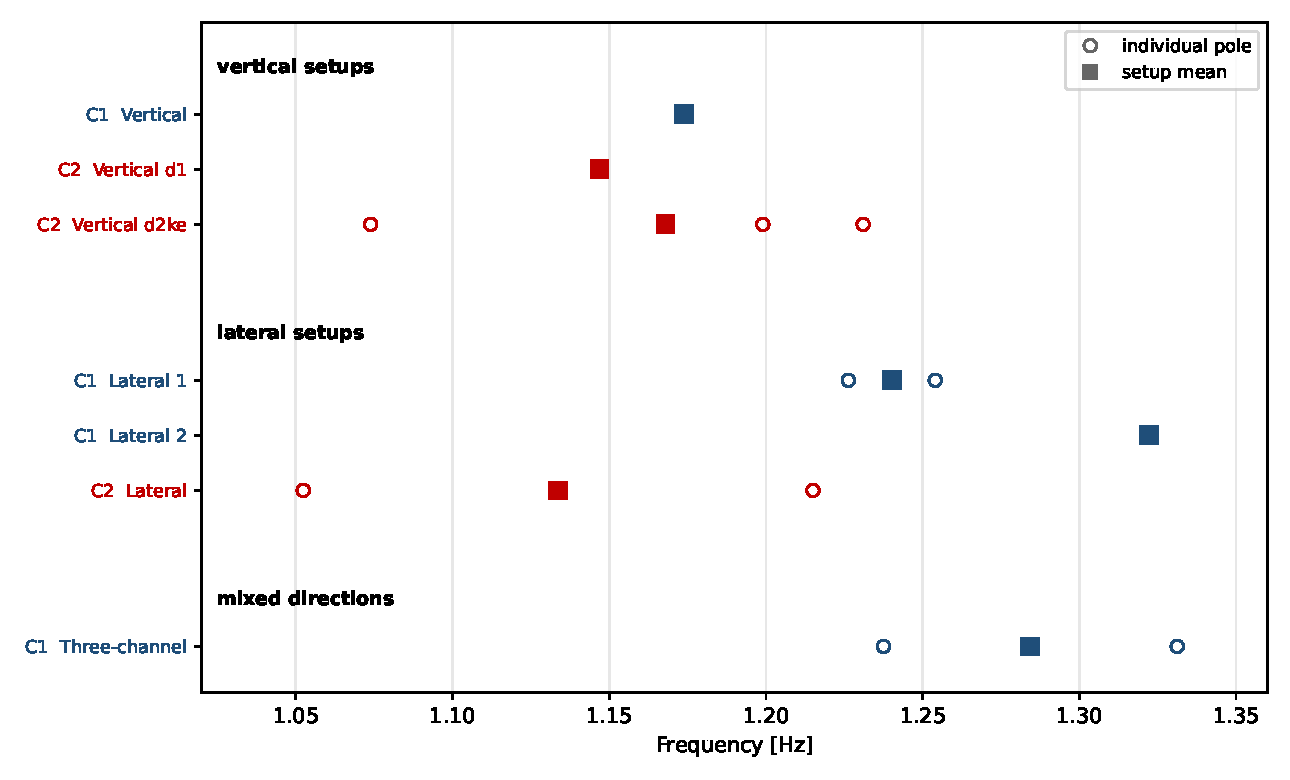
\includegraphics[width=0.85\linewidth]{fig13_frequency_shift}
\caption{Low-frequency band by setup for both campaigns, showing the individual poles and the setup means. The setup means of the two campaigns do not overlap: the smallest of campaign 1 exceeds the largest of campaign 2, a change in mean of $-8.41$\,\%. The individual poles do overlap, which is why the analysis is conducted at setup level}
\label{fig:shift}
\end{figure}

\begin{table}[htbp]
\centering
\caption{Low-band poles by setup, setup means, and the change between
campaigns.}
\label{tab:shift}
\begin{tabular}{@{}cllr@{}}
\toprule
Camp. & Setup & Poles (Hz) & Setup mean (Hz) \\
\midrule
1 & Vertical & 1.173 & 1.1734 \\
1 & Lateral 1 & 1.226, 1.254 & 1.2397 \\
1 & Lateral 2 & 1.322 & 1.3217 \\
1 & Three-channel & 1.237, 1.331 & 1.2839 \\
  & \textbf{campaign mean} & & \textbf{1.2547} \\
\midrule
2 & Lateral & 1.052, 1.215 & 1.1333 \\
2 & Vertical d1 & 1.147 & 1.1465 \\
2 & Vertical d2ke & 1.073, 1.198, 1.230 & 1.1675 \\
  & \textbf{campaign mean} & & \textbf{1.1491} \\
\midrule
  & \textbf{change} & & \textbf{$-8.41$\,\%} \\
\bottomrule
\end{tabular}
\end{table}

Applying $M_2/M_1 = (f_1/f_2)^2$ to the campaign means implies an additional
participating mass of approximately 950~tonnes, which is the correct order of magnitude for the tower, nacelle and rotor of a turbine of this class.

Three considerations support treating this as the same mode observed twice rather than as two different modes. The deformation pattern measured at the cap is the same
before and after installation. A tower fundamental mode would lie near 0.3~Hz by
soft-stiff design, a factor of four below the observed band, and the search of
Section~\ref{sec:classify} found no acceptable pole anywhere below 0.5~Hz. A change of 8\,\% is, finally, of the order expected from added mass and not of the order that separates distinct modes. The first of these is measured, the second is an
absence rather than a presence, and the third assumes what it supports; the
inference is reasonable but not proved. The figure obtained is in any case a
participating mass in this mode, not the physical mass of what was installed,
since the tower contributes rotational inertia and some stiffness as well as
mass.

% =====================================================================
\section{Conclusions}
\label{sec:conclusions}

The ordering of sway and rocking in an inclined pile group is a matter of geometry
rather than of soil. Because the two mechanisms are resisted by the same axial
pile stiffness, that stiffness cancels from the ratio of their frequencies, and
what remains depends only on the pile positions, the angle of inclination and the distribution of mass. For any inclination used in construction the
separation between the two is wide, so a single low-frequency band identified
on such a foundation may be attributed to sway without knowing the ground. The measurements confirm this: the cap translates and rotates in the pattern that sway on inclined piles produces, and the prediction and the observation are drawn from information that does not overlap. The same records also show how readily a measurement of this kind may be misinterpreted. The most prominent poles in them are not modes of the foundation. Some move a single sensor and shift when the sensors are moved. Others decay too slowly to belong to a structure and prove to be interference from the mains supply. Which of them an identification returns depends as much on the settings the analyst chooses as on the foundation itself. Acceptance was therefore made to rest on the properties a mode must possess rather than on how cleanly a pole stabilises. The criterion
itself is a first-order result. It indicates which mechanism to expect, not the frequency at which it will appear, and it should be set aside wherever a full impedance model is available. It has been demonstrated on one structure, and showing that
it discriminates correctly where the answer is already known would need a
documented benchmark. Within those limits it provides a classification obtainable from the setting-out drawing alone.

%=====================================================================
\section*{Statements and Declarations}

\paragraph{Funding} No funding was received for conducting this study.

\paragraph{Conflicts of Interest} The authors declare no conflicts of interest.

\paragraph{Author Contributions} Nguyen Hoang Bui: conceptualization, methodology, software, formal analysis, investigation, visualization, writing -- original draft. Thi Cam Nhung Nguyen: conceptualization, methodology, investigation, resources, data curation, project administration, supervision, writing -- review and editing. Huu-Quyet Nguyen: investigation, data curation. Chung Truong Thanh: software, validation. Jos\'e C. Matos: writing -- review and editing. Hung Nguyen-Dang: writing -- review and editing. All authors read and approved the final manuscript.

\paragraph{Data Availability Statement} The acceleration records analysed in this study are available from the corresponding author upon reasonable request by e-mail. The design drawings belong to the project owner and are not redistributed; every quantity read from them is given in Table~\ref{tab:geometry} and Figure~\ref{fig:section}.

\paragraph{Code Availability} The analysis is implemented in Python (NumPy, SciPy, Matplotlib). The code that regenerates every reported quantity, table and figure from the records is publicly available at \url{https://github.com/chungntu/t18-foundation-oma}.

\begin{thebibliography}{99}

\bibitem{hrennikoff1950}
Hrennikoff A (1950) Analysis of Pile Foundations with Batter Piles. Transactions of the American Society of Civil Engineers 115(1):351--374. \url{https://doi.org/10.1061/taceat.0006372}

\bibitem{saul1968}
Saul WE (1968) Static and Dynamic Analysis of Pile Foundations. Journal of the Structural Division 94(5):1077--1100. \url{https://doi.org/10.1061/jsdeag.0001945}

\bibitem{poulos1980}
Poulos HG, Davis EH (1980) Pile Foundation Analysis and Design. Wiley, New York.

\bibitem{randolph1978}
Randolph MF, Wroth CP (1978) Analysis of Deformation of Vertically Loaded Piles. Journal of the Geotechnical Engineering Division 104(12):1465--1488. \url{https://doi.org/10.1061/ajgeb6.0000729}

\bibitem{randolph1979}
Randolph MF, Wroth CP (1979) An analysis of the vertical deformation of pile groups. G{\'e}otechnique 29(4):423--439. \url{https://doi.org/10.1680/geot.1979.29.4.423}

\bibitem{mcvay1996}
McVay M, Shang T-I, Casper R (1996) Centrifuge Testing of Fixed-Head Laterally Loaded Battered and Plumb Pile Groups in Sand. Geotechnical Testing Journal 19(1):41--50. \url{https://doi.org/10.1520/gtj11406j}

\bibitem{kaynia1982}
Kaynia AM, Kausel E (1982) Dynamic stiffness and seismic response of pile groups. Research Report R82-03, Department of Civil Engineering, Massachusetts Institute of Technology, Cambridge, MA.

\bibitem{dobry1988}
Dobry R, Gazetas G (1988) Simple method for dynamic stiffness and damping of floating pile groups. G{\'e}otechnique 38(4):557--574. \url{https://doi.org/10.1680/geot.1988.38.4.557}

\bibitem{gazetas1991}
Gazetas G, Makris N (1991) Dynamic pile-soil-pile interaction. Part I: Analysis of axial vibration. Earthquake Engineering \& Structural Dynamics 20(2):115--132. \url{https://doi.org/10.1002/eqe.4290200203}

\bibitem{makris1992}
Makris N, Gazetas G (1992) Dynamic pile-soil-pile interaction. Part II: Lateral and seismic response. Earthquake Engineering \& Structural Dynamics 21(2):145--162. \url{https://doi.org/10.1002/eqe.4290210204}

\bibitem{gerolymos2008}
Gerolymos N, Giannakou A, Anastasopoulos I, Gazetas G (2008) Evidence of beneficial role of inclined piles: observations and summary of numerical analyses. Bulletin of Earthquake Engineering 6(4):705--722. \url{https://doi.org/10.1007/s10518-008-9085-2}

\bibitem{giannakou2010}
Giannakou A, Gerolymos N, Gazetas G, Tazoh T, Anastasopoulos I (2010) Seismic Behavior of Batter Piles: Elastic Response. Journal of Geotechnical and Geoenvironmental Engineering 136(9):1187--1199. \url{https://doi.org/10.1061/(asce)gt.1943-5606.0000337}

\bibitem{padron2010}
Padr{\'o}n LA, Azn{\'a}rez JJ, Maeso O, Santana A (2010) Dynamic stiffness of deep foundations with inclined piles. Earthquake Engineering \& Structural Dynamics 39(12):1343--1367. \url{https://doi.org/10.1002/eqe.1000}

\bibitem{medina2015}
Medina C, Padr{\'o}n LA, Azn{\'a}rez JJ, Maeso O (2015) Influence of pile inclination angle on the dynamic properties and seismic response of piled structures. Soil Dynamics and Earthquake Engineering 69:196--206. \url{https://doi.org/10.1016/j.soildyn.2014.10.027}

\bibitem{alamo2016}
{\'A}lamo GM, Mart{\'\i}nez-Castro AE, Padr{\'o}n LA, Azn{\'a}rez JJ, Gallego R, Maeso O (2016) Efficient numerical model for the computation of impedance functions of inclined pile groups in layered soils. Engineering Structures 126:379--390. \url{https://doi.org/10.1016/j.engstruct.2016.07.047}

\bibitem{rodriguez2025}
Rodr{\'\i}guez-Galv{\'a}n E, {\'A}lamo GM, Azn{\'a}rez JJ, Maeso O (2025) An accurate and ready-to-use approach for the estimation of impedance functions of regular pile groups for offshore wind turbine foundations. Vertical and rocking components. Engineering Structures 323:119288. \url{https://doi.org/10.1016/j.engstruct.2024.119288}

\bibitem{goit2016}
Goit CS, Saitoh M (2016) Experimental approach on the pile-to-pile interaction factors and impedance functions of inclined piles. G{\'e}otechnique 66(11):888--901. \url{https://doi.org/10.1680/jgeot.15.p.192}

\bibitem{huang2014}
Huang M, Zhong R (2014) Coupled horizontal-rocking vibration of partially embedded pile groups and its effect on resonance of offshore wind turbine structures. Chinese Journal of Geotechnical Engineering 36(2):286--294 (in Chinese). \url{https://doi.org/10.11779/CJGE201402003}

\bibitem{arany2016}
Arany L, Bhattacharya S, Macdonald JHG, Hogan SJ (2016) Closed form solution of Eigen frequency of monopile supported offshore wind turbines in deeper waters incorporating stiffness of substructure and SSI. Soil Dynamics and Earthquake Engineering 83:18--32. \url{https://doi.org/10.1016/j.soildyn.2015.12.011}

\bibitem{arany2017}
Arany L, Bhattacharya S, Macdonald J, Hogan SJ (2017) Design of monopiles for offshore wind turbines in 10 steps. Soil Dynamics and Earthquake Engineering 92:126--152. \url{https://doi.org/10.1016/j.soildyn.2016.09.024}

\bibitem{devriendt2014}
Devriendt C, Magalh{\~a}es F, Weijtjens W, De Sitter G, Cunha {\'A}, Guillaume P (2014) Structural health monitoring of offshore wind turbines using automated operational modal analysis. Structural Health Monitoring 13(6):644--659. \url{https://doi.org/10.1177/1475921714556568}

\bibitem{damgaard2013}
Damgaard M, Ibsen LB, Andersen LV, Andersen JKF (2013) Cross-wind modal properties of offshore wind turbines identified by full scale testing. Journal of Wind Engineering and Industrial Aerodynamics 116:94--108. \url{https://doi.org/10.1016/j.jweia.2013.03.003}

\bibitem{dong2018}
Dong X, Lian J, Wang H, Yu T, Zhao Y (2018) Structural vibration monitoring and operational modal analysis of offshore wind turbine structure. Ocean Engineering 150:280--297. \url{https://doi.org/10.1016/j.oceaneng.2017.12.052}

\bibitem{weijtjens2016}
Weijtjens W, Verbelen T, De Sitter G, Devriendt C (2016) Foundation structural health monitoring of an offshore wind turbine---a full-scale case study. Structural Health Monitoring 15(4):389--402. \url{https://doi.org/10.1177/1475921715586624}

\bibitem{noren2021}
Nor{\'e}n-Cosgriff K, Kaynia AM (2021) Estimation of natural frequencies and damping using dynamic field data from an offshore wind turbine. Marine Structures 76:102915. \url{https://doi.org/10.1016/j.marstruc.2020.102915}

\bibitem{tcherniak2011}
Tcherniak D, Chauhan S, Hansen MH (2011) Applicability Limits of Operational Modal Analysis to Operational Wind Turbines. In: Structural Dynamics and Renewable Energy, Volume 1. Springer New York, pp 317--327. \url{https://doi.org/10.1007/978-1-4419-9716-6_29}

\bibitem{vanvondelen2022}
van Vondelen AAW, Navalkar ST, Iliopoulos A, van der Hoek DC, van Wingerden J-W (2022) Damping identification of offshore wind turbines using operational modal analysis: a review. Wind Energy Science 7(1):161--184. \url{https://doi.org/10.5194/wes-7-161-2022}

\bibitem{peeters2001z24}
Peeters B, De Roeck G (2001) One-year monitoring of the Z24-Bridge: environmental effects versus damage events. Earthquake Engineering \& Structural Dynamics 30(2):149--171. \url{https://doi.org/10.1002/1096-9845(200102)30:2<149::aid-eqe1>3.0.co;2-z}

\bibitem{kjeld2023}
Kjeld JG, Avenda{\~n}o-Valencia LD, Vestermark J (2023) Effect of wind and wave properties in modal parameter estimates of an idling offshore wind turbine from long-term monitoring data. Mechanical Systems and Signal Processing 187:109934. \url{https://doi.org/10.1016/j.ymssp.2022.109934}

\bibitem{sastre2024}
Sastre Jurado C, Weijtjens W, Stuyts B, Winkler K, Fallais D, Devriendt C (2024) Benchmarking Measured Eigenfrequencies: A Case Study of a North Sea Offshore Wind Farm. In: Proceedings of the ASME 2024 43rd International Conference on Ocean, Offshore and Arctic Engineering (OMAE2024), Volume 5A: Ocean Engineering, V05AT06A092. \url{https://doi.org/10.1115/omae2024-125634}

\bibitem{winkler2024}
Winkler K, Sastre Jurado C, Stuyts B, Weijtjens W, Devriendt C (2024) Full-Scale Measurements of Offshore Monopile Foundations and Numerical Benchmark. In: Proceedings of the ASME 2024 43rd International Conference on Ocean, Offshore and Arctic Engineering (OMAE2024), Volume 5A: Ocean Engineering, V05AT06A090. \url{https://doi.org/10.1115/omae2024-124291}

\bibitem{nernheim2025}
Nernheim A, Voges-Espelage P, Wilsch CH, Panagoulias S, Iliopoulos A, Hermans SJ, Versteijlen P (2025) Soil modelling impact on the natural frequency of offshore wind turbines with reference to in-field measurements. In: Proceedings of the 5th International Symposium on Frontiers in Offshore Geotechnics (ISFOG 2025), Nantes, France. \url{https://www.issmge.org/uploads/publications/132/133/ISFOG2025-403.pdf}

\bibitem{fernandes2022}
Fernandes A, Winkler K, Weijtjens W, Devriendt C (2022) Operational modal analysis campaign conducted during the construction of an offshore wind farm. In: Proceedings of the International Conference on Noise and Vibration Engineering (ISMA 2022), Leuven, Belgium, pp 2695--2707.

\bibitem{seo2020}
Seo Y-H, Ryu MS, Oh K-Y (2020) Dynamic Characteristics of an Offshore Wind Turbine with Tripod Suction Buckets via Full-Scale Testing. Complexity 2020:1--16. \url{https://doi.org/10.1155/2020/3079308}

\bibitem{louw2026}
Louw H, Kearsley E (2026) Structural health monitoring of an onshore wind turbine piled-raft foundation. Structural Health Monitoring. \url{https://doi.org/10.1177/14759217251405396}

\bibitem{worldbank2021}
World Bank Group (2021) Offshore Wind Roadmap for Vietnam. Report, World Bank, Washington, DC. \url{https://documents1.worldbank.org/curated/en/261981623120856300/pdf/Offshore-Wind-Development-Program-Offshore-Wind-Roadmap-for-Vietnam.pdf}

\bibitem{nguyen2022}
Nguyen TD, Ho DA, Bui NH, Pham DH, Ngo HD, Du VT (2022) Design and Construction of Nearshore Wind Turbine Foundations: Some Experiences of APECO and FECON. In: Proceedings of the 2nd Vietnam Symposium on Advances in Offshore Engineering. Springer Singapore, pp 230--237. \url{https://doi.org/10.1007/978-981-16-7735-9_24}

\bibitem{lang2014}
Lang R, Liu R, Lian J, Ding H (2014) Study on Load-Bearing Characteristics of a New Pile Group Foundation for an Offshore Wind Turbine. The Scientific World Journal 2014:1--11. \url{https://doi.org/10.1155/2014/394104}

\bibitem{li2022}
Li Y, Wang B, Liu Q, Gao S, Lu S (2022) Application of Converted Displacement for Modal Parameter Identification of Offshore Wind Turbines with High-Pile Foundation. Journal of Ocean University of China 21(6):1467--1478. \url{https://doi.org/10.1007/s11802-022-4943-0}

\bibitem{liu2026}
Liu Y, Zhao J, Zhang L, Hu H, Yu L, Wang Y, Liu C, Luo S (2026) Dynamic Characteristics of Offshore Wind Turbine Cap-Pile Group Structure Based on Experimental Modal Analysis. In: Hydropower and Renewable Energies. Springer Nature Singapore, pp 389--397. \url{https://doi.org/10.1007/978-981-95-4889-7_33}

\bibitem{huynh2024}
Huynh QV (2024) Analysis of the dynamic behaviour of a single pile foundation when a wind turbine blade breaks. Transport and Communications Science Journal 75(6):1988--1999 (in Vietnamese). \url{https://doi.org/10.47869/tcsj.75.6.5}

\bibitem{overschee1996}
Van Overschee P, De Moor B (1996) Subspace Identification for Linear Systems. Kluwer Academic Publishers. \url{https://doi.org/10.1007/978-1-4613-0465-4}

\bibitem{peeters1999}
PEETERS B, DE ROECK G (1999) REFERENCE-BASED STOCHASTIC SUBSPACE IDENTIFICATION FOR OUTPUT-ONLY MODAL ANALYSIS. Mechanical Systems and Signal Processing 13(6):855--878. \url{https://doi.org/10.1006/mssp.1999.1249}

\bibitem{brincker2001}
Brincker R, Zhang L, Andersen P (2001) Modal identification of output-only systems using frequency domain decomposition. Smart Materials and Structures 10(3):441--445. \url{https://doi.org/10.1088/0964-1726/10/3/303}

\bibitem{reynders2012}
Reynders E (2012) System Identification Methods for (Operational) Modal Analysis: Review and Comparison. Archives of Computational Methods in Engineering 19(1):51--124. \url{https://doi.org/10.1007/s11831-012-9069-x}

\bibitem{peeters2001rev}
Peeters B, De Roeck G (2001) Stochastic System Identification for Operational Modal Analysis: A Review. Journal of Dynamic Systems, Measurement, and Control 123(4):659--667. \url{https://doi.org/10.1115/1.1410370}

\bibitem{dohler2013uq}
D{\"o}hler M, Mevel L (2013) Efficient multi-order uncertainty computation for stochastic subspace identification. Mechanical Systems and Signal Processing 38(2):346--366. \url{https://doi.org/10.1016/j.ymssp.2013.01.012}

\bibitem{zhang2005}
Zhang L, Brincker R, Andersen P (2005) An overview of operational modal analysis: major development and issues. In: Proceedings of the 1st International Operational Modal Analysis Conference (IOMAC), Copenhagen, Denmark.

\bibitem{magalhaes2009}
Magalh{\~a}es F, Cunha {\'A}, Caetano E (2009) Online automatic identification of the modal parameters of a long span arch bridge. Mechanical Systems and Signal Processing 23(2):316--329. \url{https://doi.org/10.1016/j.ymssp.2008.05.003}

\bibitem{reynders2012aoma}
Reynders E, Houbrechts J, De Roeck G (2012) Fully automated (operational) modal analysis. Mechanical Systems and Signal Processing 29:228--250. \url{https://doi.org/10.1016/j.ymssp.2012.01.007}

\bibitem{ubertini2013}
Ubertini F, Gentile C, Materazzi AL (2013) Automated modal identification in operational conditions and its application to bridges. Engineering Structures 46:264--278. \url{https://doi.org/10.1016/j.engstruct.2012.07.031}

\bibitem{neu2017}
Neu E, Janser F, Khatibi AA, Orifici AC (2017) Fully Automated Operational Modal Analysis using multi-stage clustering. Mechanical Systems and Signal Processing 84:308--323. \url{https://doi.org/10.1016/j.ymssp.2016.07.031}

\bibitem{pappa1993}
Pappa RS, Elliott KB, Schenk A (1993) Consistent-mode indicator for the eigensystem realization algorithm. Journal of Guidance, Control, and Dynamics 16(5):852--858. \url{https://doi.org/10.2514/3.21092}

\bibitem{allemang2003}
Allemang RJ (2003) The modal assurance criterion -- twenty years of use and abuse. Sound and Vibration 37(8):14--23.

\bibitem{reynders2008}
Reynders E, Pintelon R, De Roeck G (2008) Uncertainty bounds on modal parameters obtained from stochastic subspace identification. Mechanical Systems and Signal Processing 22(4):948--969. \url{https://doi.org/10.1016/j.ymssp.2007.10.009}

\bibitem{mevel2002}
MEVEL L, BASSEVILLE M, BENVENISTE A, GOURSAT M (2002) MERGING SENSOR DATA FROM MULTIPLE MEASUREMENT SET-UPS FOR NON-STATIONARY SUBSPACE-BASED MODAL ANALYSIS. Journal of Sound and Vibration 249(4):719--741. \url{https://doi.org/10.1006/jsvi.2001.3880}

\bibitem{dohler2012}
D{\"o}hler M, Mevel L (2012) Modular Subspace-Based System Identification From Multi-Setup Measurements. IEEE Transactions on Automatic Control 57(11):2951--2956. \url{https://doi.org/10.1109/tac.2012.2193711}

\bibitem{dohler2013ms}
D{\"o}hler M, Lam X-B, Mevel L (2013) Uncertainty quantification for modal parameters from stochastic subspace identification on multi-setup measurements. Mechanical Systems and Signal Processing 36(2):562--581. \url{https://doi.org/10.1016/j.ymssp.2012.11.011}

\bibitem{rainieri2014}
Rainieri C, Fabbrocino G (2014) Influence of model order and number of block rows on accuracy and precision of modal parameter estimates in stochastic subspace identification. International Journal of Lifecycle Performance Engineering 1(4):317. \url{https://doi.org/10.1504/ijlcpe.2014.064099}

\bibitem{priori2018}
Priori C, De Angelis M, Betti R (2018) On the selection of user-defined parameters in data-driven stochastic subspace identification. Mechanical Systems and Signal Processing 100:501--523. \url{https://doi.org/10.1016/j.ymssp.2017.07.045}

\bibitem{benveniste1985}
Benveniste A, Fuchs JJ (1985) Single sample modal identification of a nonstationary stochastic process. IEEE Transactions on Automatic Control 30(1):66--74. \url{https://doi.org/10.1109/tac.1985.1103787}

\bibitem{nord2019}
Nord TS, Petersen {\O}W, Hendrikse H (2019) Stochastic subspace identification of modal parameters during ice--structure interaction. Philosophical Transactions of the Royal Society A: Mathematical, Physical and Engineering Sciences 377(2155):20190030. \url{https://doi.org/10.1098/rsta.2019.0030}

\bibitem{mohanty2004}
Mohanty P, Rixen DJ (2004) Operational modal analysis in the presence of harmonic excitation. Journal of Sound and Vibration 270(1-2):93--109. \url{https://doi.org/10.1016/s0022-460x(03)00485-1}

\bibitem{brincker2000}
Brincker R, Andersen P, M{\o}ller N (2000) An indicator for separation of structural and harmonic modes in output-only modal testing. In: Proceedings of the 18th International Modal Analysis Conference (IMAC XVIII), San Antonio, TX, pp 1649--1654.

\bibitem{jacobsen2007}
Jacobsen NJ, Andersen P, Brincker R (2007) Eliminating the influence of harmonic components in operational modal analysis. In: Proceedings of the 25th International Modal Analysis Conference (IMAC XXV), Orlando, FL.

\bibitem{andersen2008}
Andersen P, Brincker R, Ventura C, Cantieni R (2008) Modal estimation of civil structures subject to ambient and harmonic excitation. In: Proceedings of the 26th International Modal Analysis Conference (IMAC XXVI), Orlando, FL.

\bibitem{jacobsen2005}
Jacobsen NJ (2005) Identifying harmonic components in operational modal analysis. In: Proceedings of the 12th International Congress on Sound and Vibration (ICSV12), Lisbon, Portugal.

\bibitem{mohanty2006}
Mohanty P, Rixen DJ (2006) Modified ERA method for operational modal analysis in the presence of harmonic excitations. Mechanical Systems and Signal Processing 20(1):114--130. \url{https://doi.org/10.1016/j.ymssp.2004.06.010}

\bibitem{le2015}
Le T-P, Argoul P (2015) Distinction between harmonic and structural components in ambient excitation tests using the time--frequency domain decomposition technique. Mechanical Systems and Signal Processing 52-53:29--45. \url{https://doi.org/10.1016/j.ymssp.2014.07.008}

\bibitem{gres2021}
Gre{\'s} S, D{\"o}hler M, Andersen P, Mevel L (2021) Kalman filter-based subspace identification for operational modal analysis under unmeasured periodic excitation. Mechanical Systems and Signal Processing 146:106996. \url{https://doi.org/10.1016/j.ymssp.2020.106996}

\bibitem{motte2015}
Motte K, Weijtjens W, Devriendt C, Guillaume P (2015) Operational Modal Analysis in the Presence of Harmonic Excitations: A Review. In: Dynamics of Civil Structures, Volume 2. Springer International Publishing, pp 379--395. \url{https://doi.org/10.1007/978-3-319-15248-6_40}

\bibitem{bk0464}
Lindahl C, Ginn B (1999) How to deal with electrical noise and interference in the measuring chain using a NEXUS conditioning amplifier. Application Note BO 0464-11, Br{\"u}el \& Kj{\ae}r, N{\ae}rum, Denmark. \url{https://www.bksv.com/media/doc/bo0464.pdf}

\bibitem{iso5348}
International Organization for Standardization (2021) ISO 5348:2021 Mechanical vibration and shock -- Mechanical mounting of accelerometers. ISO, Geneva.

\bibitem{shokrollahi2017}
Shokrollahi S, Adel F, Ahmadian H (2017) An investigation into the accelerometer mounting effects on signal transmissibility in modal measurements. Scientia Iranica 0(0):0--0. \url{https://doi.org/10.24200/sci.2017.4244}

\bibitem{abdelnour2024}
Abdelnour M, Zabel V (2023) Modal identification of structures with a dynamic behaviour characterised by global and local modes at close frequencies. Acta Mechanica 235(3):1471--1491. \url{https://doi.org/10.1007/s00707-023-03598-z}

\bibitem{bell1970}
Bell RJ, Dean P (1970) Atomic vibrations in vitreous silica. Discussions of the Faraday Society 50:55. \url{https://doi.org/10.1039/df9705000055}

\bibitem{hodges1982}
Hodges CH (1982) Confinement of vibration by structural irregularity. Journal of Sound and Vibration 82(3):411--424. \url{https://doi.org/10.1016/s0022-460x(82)80022-9}

\bibitem{pierre1987}
Pierre C, Dowell EH (1987) Localization of vibrations by structural irregularity. Journal of Sound and Vibration 114(3):549--564. \url{https://doi.org/10.1016/s0022-460x(87)80023-8}

\bibitem{en1991}
European Committee for Standardization (2010) EN 1991-1-4:2005+A1:2010 Eurocode 1: Actions on structures -- Part 1-4: General actions -- Wind actions. CEN, Brussels.

\bibitem{ohsaki1973}
Ohsaki Y, Iwasaki R (1973) On Dynamic Shear Moduli and Poisson's Ratios of Soil Deposits. Soils and Foundations 13(4):61--73. \url{https://doi.org/10.3208/sandf1972.13.4_61}

\end{thebibliography}

\end{document}
